\documentclass[12pt,oneside,a4paper,english,french,spanish,brazil,]{abntex2}

\usepackage{cmap}				% Mapear caracteres especiais no PDF
\usepackage{lmodern}			% Usa a fonte Latin Modern			
\usepackage[T1]{fontenc}		% Selecao de codigos de fonte.
\usepackage[utf8]{inputenc}		% Codificacao do documento (conversão automática dos acentos)
\usepackage{lastpage}			% Usado pela Ficha catalográfica
\usepackage{indentfirst}		% Indenta o primeiro parágrafo de cada seção.
\usepackage{color}				% Controle das cores
\usepackage{graphicx}			% Inclusão de gráficos
\usepackage{amsmath}
\usepackage{listings}
\usepackage[font=footnotesize,labelfont=bf,textfont=bf]{caption}
\usepackage[alf]{abntex2cite}	% Citações padrão ABNT
%\captionsetup[figure]{font=small}
% ---
\titulo{O USO DE ALGORITMOS GENÉTICOS PARA SEGMENTAÇÃO AUTOMÁTICA DE IMAGENS}
\autor{NÍCOLAS POHREN}
\local{Novo Hamburgo}
\data{2018}
\orientador{Marta Rosecler Bez}
\instituicao{UNIVERSIDADE FEEVALE}
\tipotrabalho{Tese (Doutorado)}
% O preambulo deve conter o tipo do trabalho, o objetivo, o nome da instituição e a área de concentração 
\preambulo{Trabalho de Conclusão de Curso apresentado como requisito parcial à obtenção do grau de Bacharel em Ciência da Computação pela Universidade Feevale}

% ---
% Configurações de aparência do PDF final

\makeatletter
\hypersetup{
     	%pagebackref=true,
		pdftitle={\@title}, 
		pdfauthor={\@author},
    	pdfsubject={\imprimirpreambulo},
	    pdfcreator={LaTeX with abnTeX2},
		pdfkeywords={abnt}{latex}{abntex}{abntex2}{trabalho acadêmico}, 
		colorlinks=true,       		% false: boxed links; true: colored links
    	linkcolor=black,          	% color of internal links
    	citecolor=black,       		% color of links to bibliography
    	filecolor=magenta,    		% color of file links
		urlcolor=blue,
		bookmarksdepth=4
}
\makeatother
% --- 

% --- 
% O tamanho do parágrafo é dado por:
\setlength{\parindent}{1.5cm}

% Controle do espaçamento entre um parágrafo e outro:
\setlength{\parskip}{0.2cm}  % tente também \onelineskip

% ---
\makeindex
% ---

% ----
\begin{document}

% 'arial' ou 'times'
%\fontemonografia{times}

% Retira espaço extra obsoleto entre as frases.
\frenchspacing 

\imprimircapa
\imprimirfolhaderosto

\imprimiragradecimento{Os agradecimentos principais são direcionados a todo mundo...}
% ---

% resumo em português
\begin{resumo}
A segmentação automática de imagens vem se tornando cada vez mais utilizada em diversas áreas como Medicina e Agronomia. Cada vez mais o método tradicional de segmentação automática, que se baseia no uso de técnicas de processamento digital de imagens, vem perdendo lugar para o uso de algoritmos baseados em redes neurais. Isso devido a sua capacidade de trabalhar com imagens pouco homogêneas. No entanto, as redes neurais acabam se tornando uma espécie de caixa-preta, onde, muitas vezes, não é possível que um ser humano interprete como o sistema chegou ao seu resultado. Neste trabalho é proposto um sistema que utiliza algoritmos genéticos para treinar o sequenciamento e a parametrização de técnicas de processamento digital de imagens. Dessa forma, espera-se demonstrar a possibilidade do sistema funcionar com imagens não homogêneas, permitindo a análise do sistema evoluído por um ser humano. Para tanto, serão realizados experimentos comparando o sistema proposto com outros semelhantes que utilizam redes neurais quanto a sua assertividade e tempo de processamento, além de validar com profissionais relacionados com a área de PDI se o sistema gerou uma saída que pode ser compreendida por seres humanos.
 \vspace{\onelineskip}
    
 \noindent
 \textbf{Palavras-chaves}: latex. abntex. editoração de texto.
\end{resumo}

% resumo em inglês
\begin{resumo}[Abstract]
 \begin{otherlanguage*}{english}
   This is the english abstract.

   \vspace{\onelineskip}
 
   \noindent 
   \textbf{Key-words}: latex. abntex. text editoration.
 \end{otherlanguage*}
\end{resumo}

% ---
\pdfbookmark[0]{\listfigurename}{lof}
\listoffigures*
\cleardoublepage
\pdfbookmark[0]{\listtablename}{lot}
\listoftables*
\cleardoublepage
% ---
\begin{siglas}
  \item[API] \textit{Application programming interface}
  \item[CMYK] \textit{Cyan, Magenta, Yellow, Black}
  \item[FA] Função de avaliação
  \item[GA] \textit{Genetic Algorithm}
  \item[HSI] \textit{Hue, Saturation, Intensity}
  \item[PDI] Processamento digital de imagens
  \item[RGB] \textit{Red, Green, Blue}
\end{siglas}
% ---
\begin{simbolos}
  \item[$ \Gamma $] Letra grega Gama
\end{simbolos}
% ---
% ---
\pdfbookmark[0]{\contentsname}{toc}
\tableofcontents*
\cleardoublepage
\textual
% ------------------------------------------------------------------------------------------------------------------------
\chapter{Introdução}
% ------------------------------------------------------------------------------------------------------------------------

Os avanços em métodos de aquisição de imagens, no poder computacional de hardware e na melhoria nas tecnologias, vêm tornando a análise automática de imagens uma técnica utilizada na resolução de diversos problemas. Destaca-se o uso da análise de imagens nas áreas da Medicina, Biologia, Sensoriamento Remoto, Meteorologia, Automação Industrial, Engenharia, Geologia e Agronomia \cite{queiroz:2007}.  

Um problema comum de análise de imagens é a segmentação destas. O processamento para segmentação de imagens visa identificar e separar a imagem em diferentes regiões relevantes para o processamento em questão. Como exemplo é possível citar a segmentação de órgãos, como pulmões, em um exame de tomografia computadorizada \cite{ronnau:2015}.

Uma forma de realizar a análise das imagens se dá pela execução de uma sequência de algoritmos de processamento digital de imagens (PDI) \cite{gonzalez:2012}. Esses algoritmos podem ser orquestrados e parametrizados pelo criador do sistema, ou de forma empírica pelo usuário. Mais recentemente, outra forma utilizada para a resolução de problemas de segmentação e classificação de imagens é a aplicação de redes neurais (RN) simples ou convolucionais \cite{noh:2015}, onde um sistema de aprendizado de máquina é treinado para executar a tarefa especificada. Esse treinamento é efetuado de forma supervisionada, necessitando de uma base previamente anotada, o que é um recurso de construção bastante custoso.

A técnica de RN vem ganhando visibilidade no mundo acadêmico. Isso se deve a diversos fatores. O uso de RN permite que um único sistema seja treinado para solucionar diversos problemas. Também é possível que o treinamento supervisionado da RN seja realizado por um especialista no assunto em questão e que não necessite de conhecimento do sistema e da tecnologia utilizada. Além disso, o seu resultado normalmente é superior quando as imagens não são homogêneas, ou seja, não se enquadram perfeitamente na situação prevista pelo sistema \cite{pal:1993}.

No entanto, sistemas baseados em redes neurais oneram em tempo de processamento em relação aos sistemas baseados em PDI \cite{huang:1992}, o que pode ser um problema para sistemas de monitoramento em tempo real ou avaliação de uma grande quantidade de imagens.

Embora existam tentativas anteriores de analisar e compreender a saída de uma RN \cite{zeiler:2014}, isso não é possível em todas as soluções que utilizam RN. Dessa forma, arede neural acaba se tornando uma caixa-preta, de forma que geralmente não é possível a um ser humano interpretar como ela está chegando ao resultado de forma que ele possa aprender com o sistema e reproduzir os resultados.

Em outras soluções desenvolvidas para problemas específicos são utilizadas técnicas de PDI pré-selecionadas e algoritmos genéticos \cite{holland:1992} para o treinamento dos seus parâmetros. Pode-se citar o software que segmenta elementos em fotos de satélite \cite{costa:2010} ou a comparação da evolução dos parâmetros em métodos de segmentação baseados em \textit{quadtrees}, \textit{thresholding} e crescimento de regiões \cite{matias:2007}. Entretanto, todos os trabalhos utilizam o AG apenas para ajustar os parâmetros dos algoritmos de PDI, sem tentar utilizar o AG para mudar o algoritmo a ser utilizado ou a sequência de passos para obter o resultado.

Propõe-se, neste trabalho, um sistema que seja capaz de utilizar algoritmos genéticos tanto para parametrizar quanto para sequenciar técnicas de PDI de acordo com a imagem. Acredita-se que isso permitirá a obtenção de resultados de qualidade semelhante a de redes neurais, porém, com uma tempo de processamento inferior . Esta abordagem também permitirá o estudo por parte de um ser humano para interpretar a sequência de passos utilizada, de forma a aprender e refinar o processamento.

Prévio a escrita deste projeto, foi desenvolvido um ambiente de manipulação de técnicas de PDI denominado VISNode \cite{visnode:2018}. Este permite a utilização e parametrização de processos de PDI em formato de grafo, onde os processos não são executados necessariamente em sequência, e parâmetros podem ser transferidos entre processos, ou nodos. A ferramenta permite a execução dos grafos de processos, denominados projetos, via uma \textit{application programming interface} (API) utilizando como entrada um conjunto de imagens, assim como a visualização destes projetos em uma interface gráfica.

Com base neste ambiente, o sistema proposto terá como saída um projeto da ferramenta VISNode. Assim, será possível visualizar facilmente os processos que estão sendo utilizados, em que sequência e com quais parâmetros, pela interface do sistema.

% TODO: No capiútlo X....

% ------------------------------------------------------------------------------------------------------------------------
\chapter{Algoritmos Genéticos}
% ------------------------------------------------------------------------------------------------------------------------

Este capítulo trata da técnica de algoritmos genéticos (do inglês \textit{genetic algorithms}, ou GA). São apresentados os conceitos de população, geração, cromossomos, genes, \textit{crossover} e mutação.

\section{Algoritmos Evolucionários}

Na área de inteligência artificial, algoritmos evolucionários usam modelos computacionais dos processos naturais de evolução como uma ferramenta para resolver problemas de otimização. Apesar de haver uma grande variedade de modelos computacionais propostos, todos eles têm em comum o conceito de simulação da evolução das espécies através de seleção, mutação e reprodução, processos estes que dependem do desempenho dos indivíduos desta espécie dentro do seu ambiente \cite{linden:2008}.

Os algoritmos evolucionários funcionam mantendo uma população de estruturas, denominadas de indivíduos, cada um representando uma solução para o problema. Cada indivíduo recebe uma avaliação, que é uma qualificação de sua qualidade como solução do problema em questão. Esta avaliação é calculada utilizando uma função de avaliação (FA ou \textit{fitness function}). Com base nesta avaliação são aplicados operadores que simulam conceitos da biologia, como reprodução e mutação, de forma a simular a sobrevivência do mais apto \cite{linden:2008}.

O primeiro passo para um algoritmo evolucionário é a criação da população inicial, chamado de primeira geração. O tamanho de uma população varia de acordo com o problema, mas é comum se utilizar populações de centenas ou milhares de indivíduos. Normalmente esta geração é completamente aleatória para garantir a máxima diversidade nos indivíduos \cite{linden:2008}.

Após a criação da primeira geração, cada indivíduo é avaliado de acordo com a função de avaliação. A FA é utilizada para avaliar e sumarizar o quão próximo cada indivíduo está de alcançar o seu objetivo. A definição da função de avaliação é o passo mais importante para a criação de um algoritmo evolucionário, pois é ela quem dita o objetivo do algoritmo. Muitas vezes não é possível calcular diretamente a função de avaliação de um indivíduo, sendo necessária a realização de uma simulação para obter o seu valor \cite{linden:2008}.

Seleciona-se então os indivíduos com a maior avaliação para reprodução. Uma nova população (próxima geração) é criada com base nos indivíduos mais aptos da geração anterior. Podem ser utilizados diversos operadores para a criação dos novos indivíduos, como \textit{crossover} (reprodução) e mutação. Ao fim do processo, existirá uma nova população, que deverá ser avaliada novamente e o processo se repete para a criação da próxima geração.

Este processo é executado até que uma condição de terminação seja atingida. Essa condição de terminação pode ser o alcance de uma avaliação mínima, número de gerações ou quantidade de recursos de processamento utilizados.

\section{Algoritmos Genéticos}

Algoritmos genéticos são um ramo dos algoritmos evolucionários que traz conceitos da biologia genética como genes e cromossomos para os algoritmos evolucionários. Isso permite a melhor simulação de um sistema evolucionário próximo ao que existe na natureza, obtendo resultados de alta qualidade para problemas de otimização.

Como os algoritmos genéticos fazem parte do grupo de algoritmos evolucionários, eles possuem a mesma sequência de passos: inicialização, avaliação, simulação e criação de uma nova geração. O diferencial do algoritmo genético é o uso de cromossomos para representar um indivíduo. O cromossomo é uma sequência de valores, ou genes, que representa a solução daquele indivíduo.

Para a criação das novas gerações, são utilizadas funções com base nos cromossomos. Alguns exemplos de operadores são o \textit{crossover}, que visa juntar dois cromossomos pais para criação de cromossomos filhos que herdam características de seus pais, e o operador de mutação, que simula a possibilidade natural de uma mutação genética. O fluxo de um algoritmo genético pode ser visto na Figura~\ref{fig:GA_Fluxo}.

\begin{figure}[ht]
\centering
\caption{Fluxo básico de um algoritmo genético}
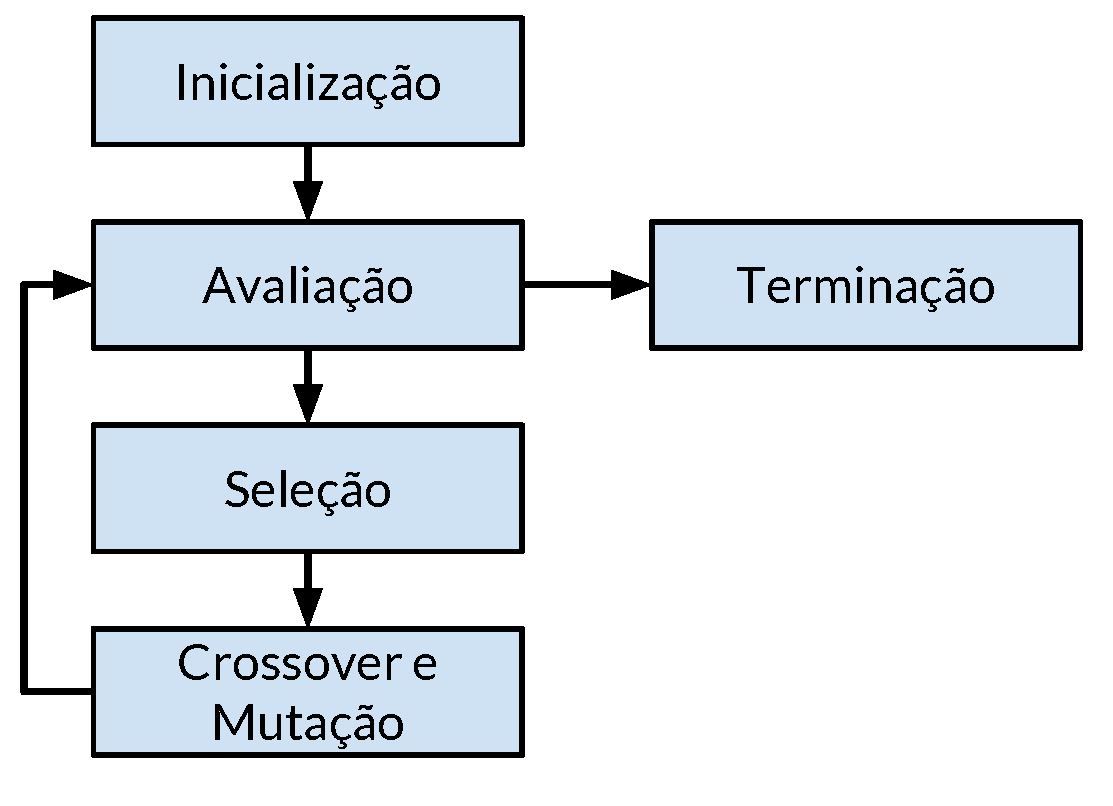
\includegraphics[width=0.5\textwidth]{imagens/GA_Fluxo.pdf}
\source{Adaptado de \citet{linden:2008}}
\label{fig:GA_Fluxo}
\end{figure}

\subsection{Representação Cromossomial}

Em algoritmos genéticos todos os indivíduos são representados por uma cadeia de valores chamada de cromossomo. Cada pedaço indivisível desta representação é chamado de gene, por analogia com as partes fundamentais que compõem um cromossomo biológico.

A codificação da informação em cromossomos é um ponto crucial dentro do GA, e é, junto com a função de avaliação, o que liga o GA ao problema a ser resolvido. Se a codificação for feita de forma inteligente, esta já incluirá as idiossincrasias do problema e permitirá que se evitem testes de viabilidade de cada uma das soluções geradas \cite{linden:2008}.

A representação mais simples e mais usada pelos praticantes da área de algoritmos genéticos é a binária, isto é, um cromossomo nada mais é do que uma sequência de \textit{bits}. Essa representação foi adotada inicialmente por \citet{holland:1992} e, hoje em dia, ela é amplamente adotada por pesquisadores da área de GA. Ademais, os operadores genéticos são compreensíveis e implementáveis rapidamente para cromossomos binários \cite{linden:2008}.

Um cromossomo para o algoritmo genético é apenas uma sequência de valores individuais. O GA não sabe a natureza do problema que o indivíduo está tentando solucionar. Quem fará a ligação do cromossomo com o problema será a função de avaliação, que será descrita mais detalhadamente na seção~\ref{sec:Funcao_de_Avaliacao}. Um exemplo de representação cromossomial binária pode ser um cromossomo de três genes, onde o primeiro gene representa a cor vermelha, o segundo a cor verde e o terceiro a cor azul. Assim, na Figura~\ref{fig:GA_Cromossomo_RGB}, é possível ver todo o espaço de soluções representáveis por este cromossomo.

\begin{figure}[ht]
\centering
\caption{Todas as variações possíveis de um cromossomo cujos bits 0, 1 e 2 representam o estado das cores vermelho, azul e verde respectivamente}
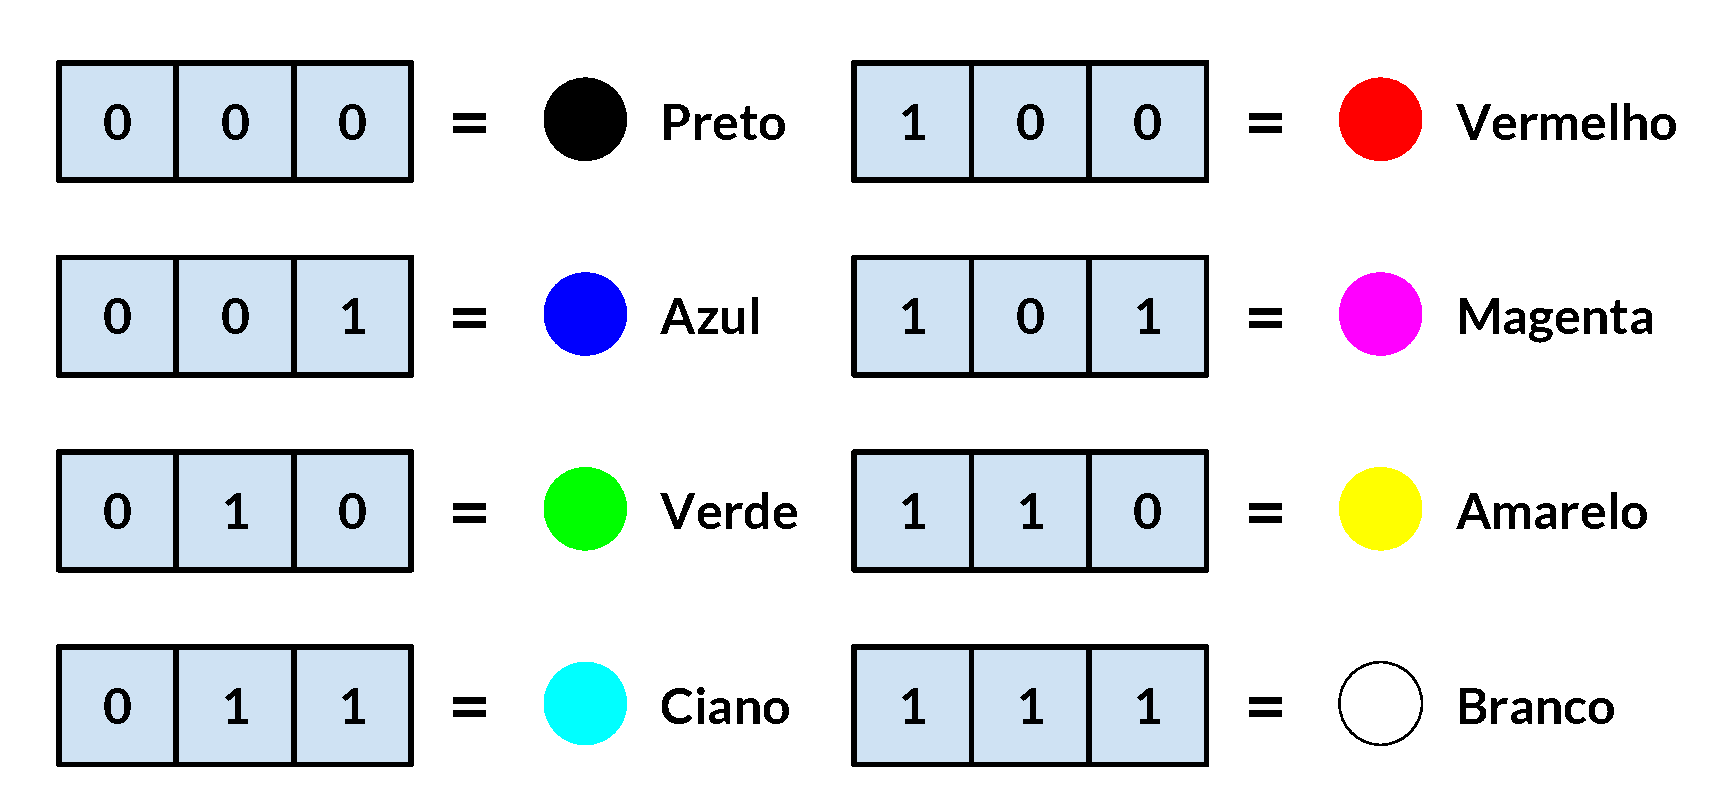
\includegraphics[width=0.8\textwidth]{imagens/GA_Cromossomo_RGB.pdf}
\sourceAuthor	
\label{fig:GA_Cromossomo_RGB}
\end{figure}

No entanto, a representação binária tem dificuldades ao lidar com múltiplas dimensões de variáveis contínuas, principalmente com alta precisão. Esta também não é uma representação ideal quando existe um número finito de estados distintos que não é múltiplo de dois, pois muitos estados se tornarão inválidos. Por esta razão existem outras formas de representação cromossomial, como a numérica e a categórica.

A representação cromossomial numérica assume que cada gene terá um valor inteiro ou real ao invés de valores binários. Outra forma de representação cromossomial é a categórica, onde cada gene representa um valor de uma lista de valores possíveis.

Ainda existe a possibilidade da criação de um cromossomo híbrido. Em um cromossomo de representação híbrida, cada gene pode ter a sua própria representação (binária, numérica ou categórica), e os operadores genéticos devem funcionar de acordo com o tipo do gene \cite{linden:2008}.

\subsection{Inicialização}

O primeiro passo de um algoritmo genético é a criação da geração inicial. Neste passo é criada uma população de indivíduos, sendo que cada indivíduo possui o seu cromossomo como uma cadeia completamente aleatória de genes. A lei das probabilidades sugere que existirá uma distribuição de soluções que cobre praticamente todo o espaço de soluções, mas isto não pode ser garantido, pois a população possui um tamanho finito \cite{linden:2008}.

O desempenho do algoritmo genético é extremamente sensível ao tamanho da população, logo, este parâmetro deve ser definido com muito cuidado. Caso este número seja pequeno demais, não haverá espaço para uma variedade genética suficientemente grande dentro da população, o que fará com que o algoritmo seja incapaz de achar boas soluções. Caso este número seja grande demais, o algoritmo demorará demais e utilizará muitos recursos computacionais  \cite{linden:2008}. Normalmente populações variam entre centenas e milhares de indivíduos.

\subsection{Função de Avaliação}
\label{sec:Funcao_de_Avaliacao}

Segundo \citet{linden:2008}, a função de avaliação é a maneira utilizada pelos GAs para determinar a qualidade de um indivíduo como solução do problema em questão. A FA pode ser considerada como uma nota numérica dada ao indivíduo na resolução do problema. Essa avaliação será utilizada para a escolha dos indivíduos pelo módulo de seleção dos pais, sendo a forma de diferenciar entre as boas e as más soluções para um problema.

GAs são técnicas de maximização, logo, a função de avaliação deve ser tal que se o cromossomo C1 representa uma solução melhor que o cromossomo C2, então a avaliação de C1 deve ser maior do que a avaliação de C2. A função de avaliação deve refletir os objetivos a serem alcançados na resolução de um problema e é derivada diretamente das condições impostas por este problema \cite{holland:1992}.

Um cuidado a ser tomado com a função de avaliação é o problema do super indivíduo. Este problema ocorre quando há um ou mais indivíduos cuja avaliação é muito superior àquela dos outros membros da população. Neste caso, este indivíduo será quase sempre escolhido pelo módulo de seleção, causando uma perda imediata da diversidade genética nas gerações subsequentes.

Para solucionar este problema, é possível utilizar outras técnicas como a de normalização linear. A normalização de uma função de avaliação funciona atribuindo um valor constante \(k\) ao melhor cromossomo, \(k - c\) para o segundo indivíduo, \(k - 2c\) para o terceiro indivíduo, e assim sucessivamente, sendo \(k\) e \(c\) duas constantes definidas pelo criador do GA. Com a normalização, os indivíduos permanecerão na mesma ordem de avaliação, mas com um intervalo constante entre eles  \cite{linden:2008}. Um exemplo de normalização pode ser visto no Quadro~\ref{tab:Normalizacao_Avaliacao}, utilizando as constantes \(k = 10\) e \(c = 1\).

\begin{table}[tbp]
\centering
\caption{Exemplo de avaliações e normalização}
\label{tab:Normalizacao_Avaliacao}
\begin{tabular}{rrr}
\hline
\multicolumn{1}{l}{\textit{\textbf{Indivíduo}}} & \multicolumn{1}{l}{\textit{\textbf{Avaliação}}} & \multicolumn{1}{l}{\textit{\textbf{Avaliação normalizada}}} \\ \hline
0                                                & 123,48                                           & 10                                                           \\
1                                                & 68,42                                            & 9                                                            \\
2                                                & 18,45                                            & 8                                                            \\
3                                                & 18,38                                            & 7    \\ \hline                                                       
\end{tabular}
\end{table}

\subsection{Seleção}

O próximo passo é a criação de uma nova população para a próxima geração. A população da nova geração será criada com base nos indivíduos da população anterior e os operadores de \textit{crossover} e mutação. Normalmente a população da nova geração terá um tamanho idêntico a população anterior \cite{linden:2008}.

Para cada indivíduo a ser criado na nova população são selecionados dois ou mais indivíduos da geração anterior com base em sua função de avaliação. Esses dois indivíduos servirão como pais do novo cromossomo. Com base nos operadores de \textit{crossover} e mutação, o novo indivíduo tipicamente possuirá várias características de seus pais. Novos pares de pais são selecionados para cada novo indivíduo, de forma que quanto maior a avaliação de um indivíduo, maior é sua chance de ser selecionado como pai \cite{linden:2008}. Também é possível utilizar métodos que usam mais de dois indivíduos como pais, o que não é tão análogo com a reprodução natural, mas algumas pesquisas indicam que o resultado é superior \cite{ting:2005} \cite{eiben:1994}.

O método mais comum para seleção de pais é o da roleta viciada. Para a realização deste método, é atribuída uma probabilidade para cada indivíduo \(p_i = p_i-1 + \frac{a}{t}\), sendo \(a\) a avaliação daquele indivíduo e \(t\) a soma de todas as avaliações. Dessa forma, a soma de todas as probabilidades deverá ser 1 (ou 100\%). É sorteado então um número aleatório \(r\) entre 0 e 1 e selecionado o indivíduo onde \(p_i-1 < r < p_i\). Dessa forma, quanto maior a avaliação de um indivíduo, maior sua chance de ser selecionado \cite{linden:2008}. Um exemplo de uma distribuição de roleta viciada pode ser visto no Quadro~\ref{tab:Roleta}.

\begin{table}
\centering
\caption{Exemplo de roleta viciada}
\label{tab:Roleta}
\begin{tabular}{lll}
\hline
\textit{\textbf{Indivíduo}} & \textit{\textbf{Avaliação}} & \textit{\textbf{Pedaço da roleta (\%)}} \\ \hline
0001      & 1         & 1.61                  \\
0011      & 9         & 14.51                 \\ 
0100      & 16        & 25.81                 \\ 
0110      & 36        & 58.07                 \\ 
Total     & 62        & 100                   \\ \hline
\end{tabular}
\end{table}

Ao final deste processo existirá uma nova população que é diferente da geração inicial. A chance de que a avaliação média desta geração seja maior ou pelo menos igual a média da geração anterior é superior a chance de ser inferior. Isso se deve ao fato de apenas os indivíduos mais aptos terem sido selecionados para a reprodução \cite{linden:2008}.

Os indivíduos com uma avaliação menor ainda devem ter chance de serem selecionados para reprodução, embora menor, o que garante uma diversidade genética maior entre a população. Uma maior diversidade genética é importante para garantir que um espectro maior de soluções sejam exploradas pelo algoritmo.

\subsection{Operadores Genéticos}

Os operadores genéticos são funções aplicadas sobre um ou mais cromossomos para a geração de novos cromossomos. Os exemplos mais simples de operadores genéticos são o \textit{crossover} e a mutação. O operador de \textit{crossover} é o responsável por gerar um novo cromossomo baseado em dois cromossomos pais. O operador de mutação é aplicado em um cromossomo para que ele tenha uma pequena chance de sofrer uma mutação genética em algum gene. Existe mais de uma técnica de \textit{crossover} e mutação, ambas podem ser parametrizadas e podem ou não ser executadas.

A técnica de \textit{crossover} mais simples é o \textit{crossover} de um ponto. No \textit{crossover} de um ponto são usados dois cromossomos pais para gerar dois cromossomos filhos. Para realizar um \textit{crossover} de um ponto, é selecionada uma posição aleatória do cromossomo, e ambos os cromossomos pais são cortados nesta posição. O primeiro filho é composto através da concatenação da parte esquerda do primeiro pai com a parte direita do segundo pai. O segundo filho é composto através da concatenação das partes que sobraram, ou seja, a metade esquerda do segundo pai com a metade à direita do primeiro pai \cite{linden:2008}. É possível ver, na Figura~\ref{fig:GA_Crossover_de_um_ponto}, um exemplo de \textit{crossover}  de um ponto sendo executado em um cromossomo de tamanho cinco com representação binária.

\begin{figure}[ht]
\centering
\caption{Exemplo de um \textit{crossover} de um ponto. a) Os dois pais utilizados para a operação de \textit{crossover}; b) O ponto de corte selecionado aleatoriamente; c) Os dois filhos gerados pelo operador de \textit{crossover}}
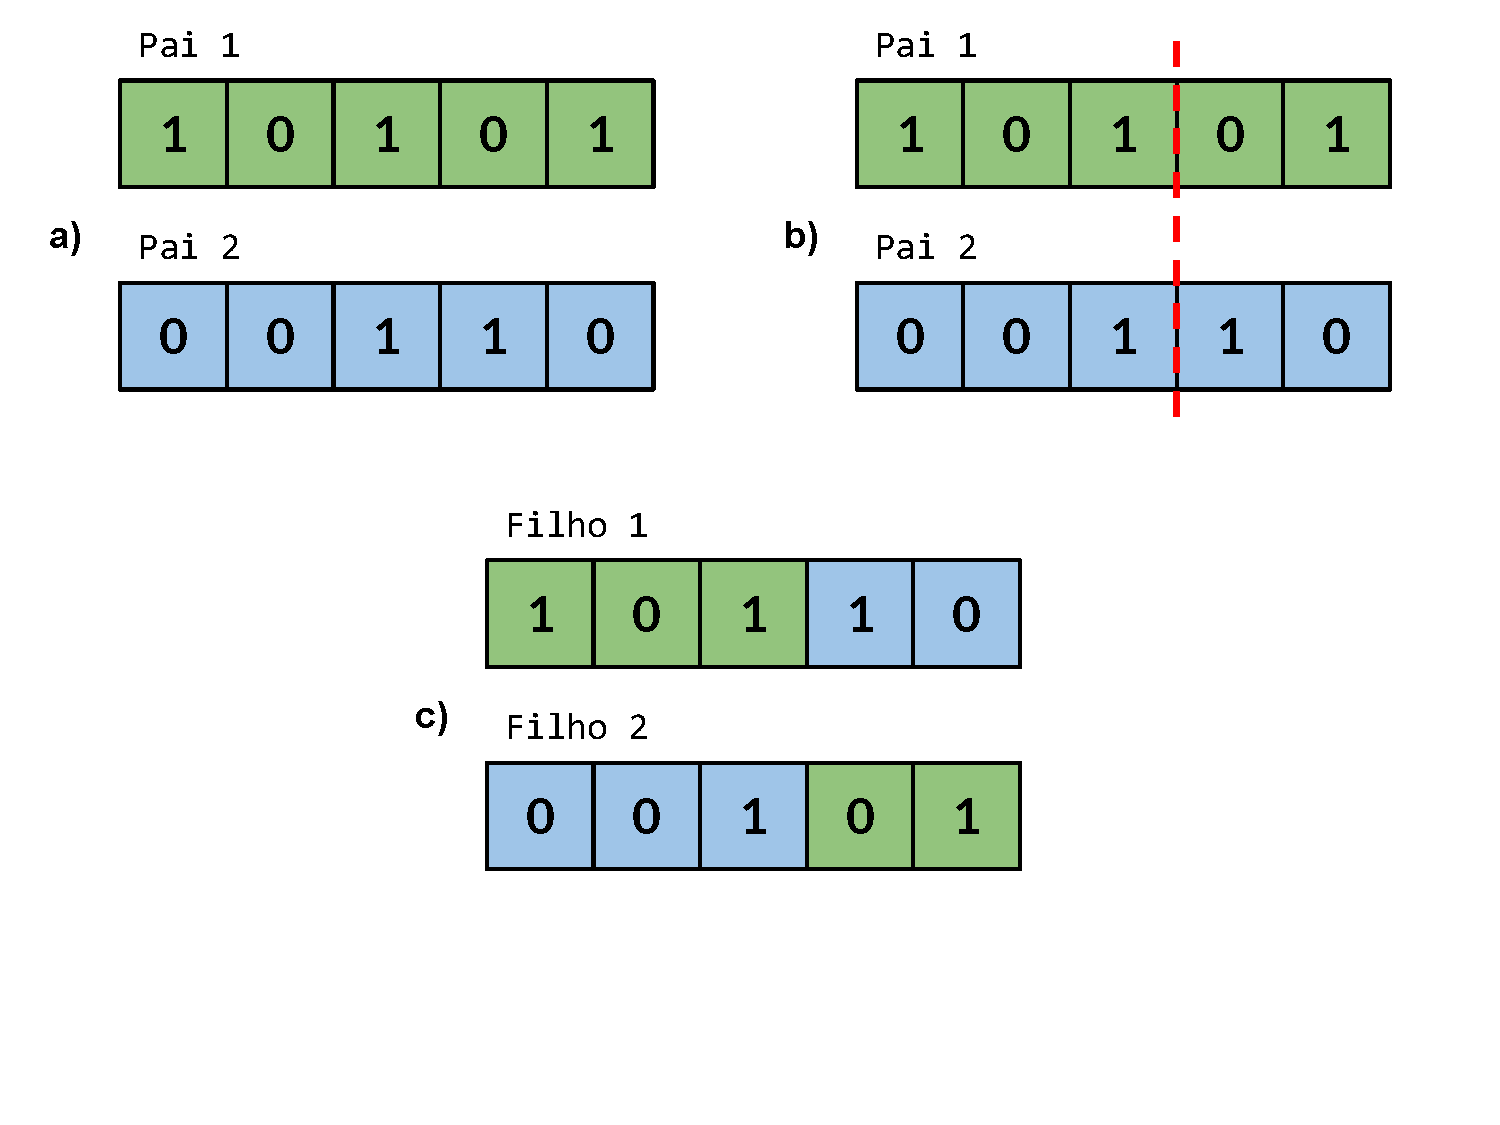
\includegraphics[width=0.7\textwidth]{imagens/GA_Crossover_de_um_ponto.pdf}
\source{Adaptado de \citet{linden:2008}}
\label{fig:GA_Crossover_de_um_ponto}
\end{figure}

Um problema gerado por um \textit{crossover} de um ponto é que se a combinação de melhor resultado depende que, por exemplo, o primeiro e o último gene sejam 1 (denominado de esquema 1 * * * 1 para um cromossomo de 5 genes), essa combinação pode não ser preservada no \textit{crossover}. Isso se deve ao fato de que pelo menos uma das duas metades do cromossomo será trocada com outro indivíduo, e se o indivíduo não tiver essa combinação, então este esquema será perdido \cite{linden:2008}.

Existe outra forma de operação de \textit{crossover} que possibilita a preservação de tais esquemas, chamada de \textit{crossover} uniforme. No \textit{crossover} uniforme, para cada gene é sorteado um número zero ou um. Se o valor for igual a um, o filho número um recebe o gene da posição corrente do primeiro pai e o segundo filho o gene corrente do segundo pai. Por outro lado, se o valor sorteado for zero, as atribuições serão invertidas: o primeiro filho recebe o gene da posição corrente do segundo pai e o segundo filho recebe o gene corrente do primeiro pai \cite{linden:2008}. Na Figura~\ref{fig:GA_Crossover_Uniforme} é possível ver o funcionamento do \textit{crossover} uniforme, com um cromossomo de cinco bits.

\begin{figure}[ht]
\centering
\caption{Exemplo de \textit{crossover} uniforme. a) Par de pais selecionados para o \textit{crossover}; b) Seleção aleatória binária para cada gene; b) Construção do par de filhos utilizando o par de pais e o conjunto binário que define de qual pai o gene de cada filho virá}
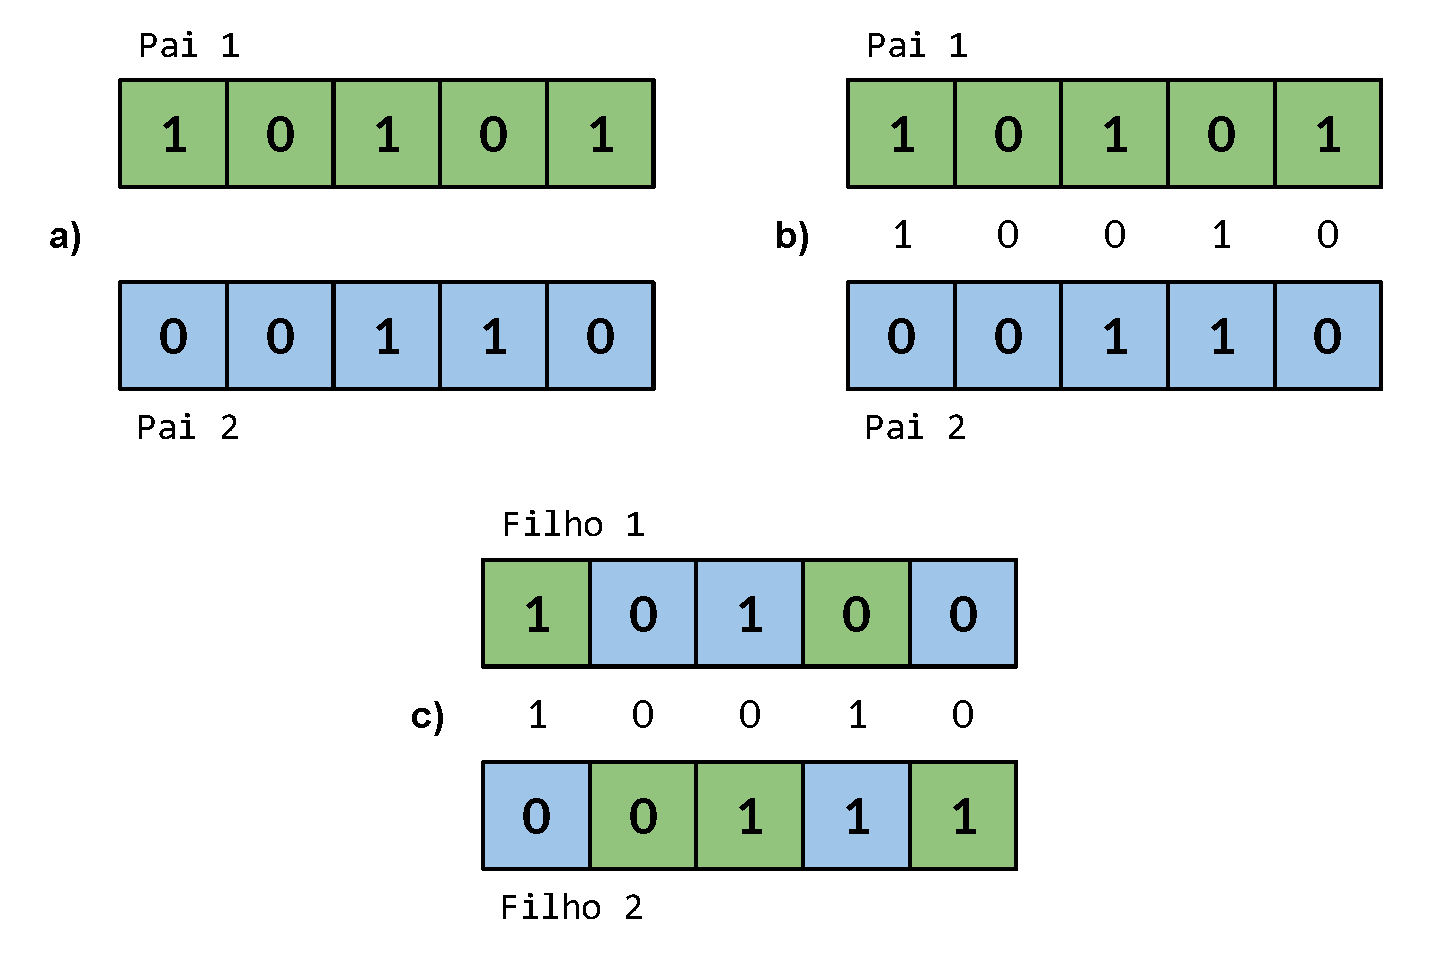
\includegraphics[width=0.7\textwidth]{imagens/GA_Crossover_Uniforme.pdf}
\source{Adaptado de \citet{linden:2008}}
\label{fig:GA_Crossover_Uniforme}
\end{figure}

Outro operador utilizado na criação de uma nova geração é o operador de mutação. O objetivo do operador de mutação é incrementar a diversidade genética da população durante a execução do algoritmo, para explorar possibilidades que não foram concebidas na geração inicial e que não foram obtidas com o operador de \textit{crossover}. O operador de mutação opera em cada gene do cromossomo, e possui uma chance normalmente muito baixa (da ordem de 0,5\%) de alterar o valor do gene em questão. Para um gene binário, o operador de mutação inverterá o bit em questão, como demonstrado na Figura~\ref{fig:GA_Mutacao}, para genes numéricos ou categóricos, um novo valor totalmente aleatório será escolhido \cite{linden:2008}.

\begin{figure}[ht]
\centering
\caption{Exemplo de um operador de mutação em um cromossomo de cinco bits}
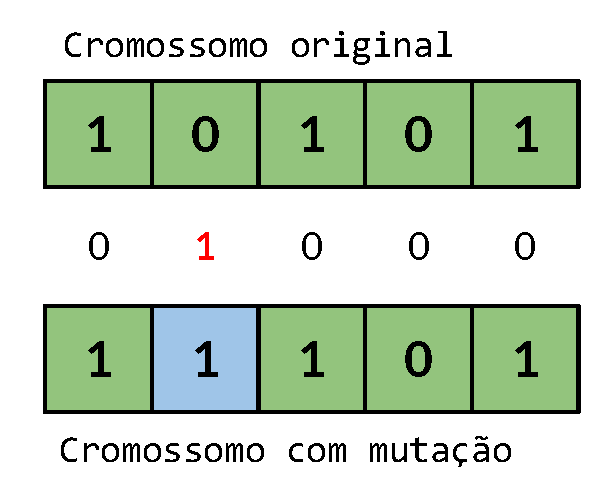
\includegraphics[width=0.4\textwidth]{imagens/GA_Mutacao.pdf}
\source{Adaptado de \citet{linden:2008}}
\label{fig:GA_Mutacao}
\end{figure}

Anteriormente foi demonstrado o operador de \textit{crossover} para genes binários. Para genes numéricos, o operador de mutação ocorre trocando um gene por um novo valor completamente aleatório. Já para valores categóricos, deve ser garantido que todas as categorias tenham o mesmo peso ou chance de serem obtidas \cite{linden:2008}.

Normalmente os operadores de \textit{crossover} e mutação não são executados em todos os indivíduos de todas gerações. No início do GA, é desejável executar muita reprodução e pouca mutação, visto que há muita diversidade genética e é importante explorar o máximo possível o espaço de soluções. Depois de um grande número de gerações, ocorre a convergência genética, o que implica na pouca diversidade na população, tornando extremamente interessante que o operador de mutação fosse escolhido mais frequentemente do que o de \textit{crossover}, para permitir que seja reinserida a diversidade genética na população \cite{linden:2008}.

Seria necessário então que a probabilidade do operador de \textit{crossover} fosse caindo com o decorrer do algoritmo e que a probabilidade do operador de mutação fosse concomitantemente aumentando. Para tal, são utilizadas diversas técnicas de interpolação, como a linear, quadrática e descontínua \cite{linden:2008}.

\section{Considerações}

Este capítulo apresentou a técnica de algoritmos genéticos como uma poderosa ferramenta para a otimização de problemas. Foram demonstrados os seus principais conceitos, como população, geração, \textit{fitness}, indivíduo, gene e cromossomo, tal como as técnicas utilizadas, entre elas a mutação, \textit{crossover} de um ponto e \textit{crossover} uniforme.

No próximo capítulo serão apresentadas técnicas de processamento digital de imagens. O uso destas técnicas para segmentação de imagens será considerado como um problema de otimização global, o qual será resolvido utilizando algoritmos genéticos.


% ------------------------------------------------------------------------------------------------------------------------
\chapter{Análise e processamento de imagens digitais}
\label{chp:PDI}
% ------------------------------------------------------------------------------------------------------------------------

Este capítulo aborda o tema sobre processamento digital de imagens. Serão explicados os conceitos de imagem digital, pré-processamento e segmentação, tal como diversas técnicas para análise e manipulação de imagens.

Segundo \citet{pedrini:2008}, o processamento digital de imagens consiste em um conjunto de técnicas para capturar, representar e transformar imagens com o auxílio do computador. O emprego dessas técnicas permite extrair e identificar informações das imagens e melhorar a qualidade visual de certos aspectos estruturais, facilitando a percepção humana e a interpretação automática por meio de máquinas. 

\citet{conci:2003} definem uma imagem digital como um conjunto finito de pontos que são representados por um número finito e discreto de tons ou cores. A representação adequada de uma imagem em tons de cinza é como uma matriz bidimensional cujas linhas e colunas identificam um ponto na imagem. Cada ponto, também chamado de pixel, é representado no computador como um número inteiro que corresponde a intensidade de luz no ponto. Frequentemente, a cor do pixel é representada como um inteiro de 8 bits variando entre 0 e 255, sendo o valor 0 correspondente à cor preta, 255 à cor branca, e as outras tonalidades de cinza distribuídas entre esses valores limites.

Nessa representação de uma imagem como uma matriz de pixels bidimensional, os índices da matriz são valores inteiros que especificam a linha e a coluna na matriz. O pixel (0,0) está localizado no canto superior esquerdo da imagem. As posições dos pontos no plano da imagem têm coordenadas \(x\) e \(y\). A coordenada \(y\) corresponde à direção vertical, e a coordenada \(x\) corresponde à direção horizontal. O eixo \(y\) é positivo para baixo e o eixo \(x\) positivo para a direita. Assim, o valor de cada pixel é representado pela função \(f(x,y)\).

Ao trabalhar com imagens coloridas, é utilizado um conjunto de planos bidimensionais para representar diferentes cores ou propriedades da imagem, onde cada plano é denominado canal. O modelo de representação mais comum para imagens é o RGB, onde cada plano bidimensional da imagem representa, respectivamente, Vermelho (\textit{Red}), Verde (\textit{Green}) e Azul (\textit{Blue}). Outros modos de representação bastante utilizados são CMYK (\textit{Cyan}, \textit{Magenta}, \textit{Yellow} e \textit{Black}) e HSI (\textit{Hue}, \textit{Saturation} e \textit{Intensity}). Em todas as representações ainda é possível adicionar um novo canal, denominado Alpha, que serve para representar a transparência do pixel.

Segundo \citet{pedrini:2008}, um sistema de processamento digital de imagens é constituído por um conjunto de cinco etapas, representados na Figura~\ref{fig:PDI_Etapas_PDI}, capazes de produzir um resultado a partir do domínio do problema. As etapas são: aquisição; pré-processamento; segmentação; representação e reconhecimento. Todo o conhecimento sobre o domínio do problema está codificado na forma de uma base de conhecimento. Esta é dependente da aplicação, cujo tamanho e complexidade podem variar significativamente. A base de conhecimento é utilizada para guiar a comunicação entre os módulos de processamento a fim de executar uma determinada tarefa.

\begin{figure}[ht]
\centering
\caption{Etapas do processamento digital de imagens}
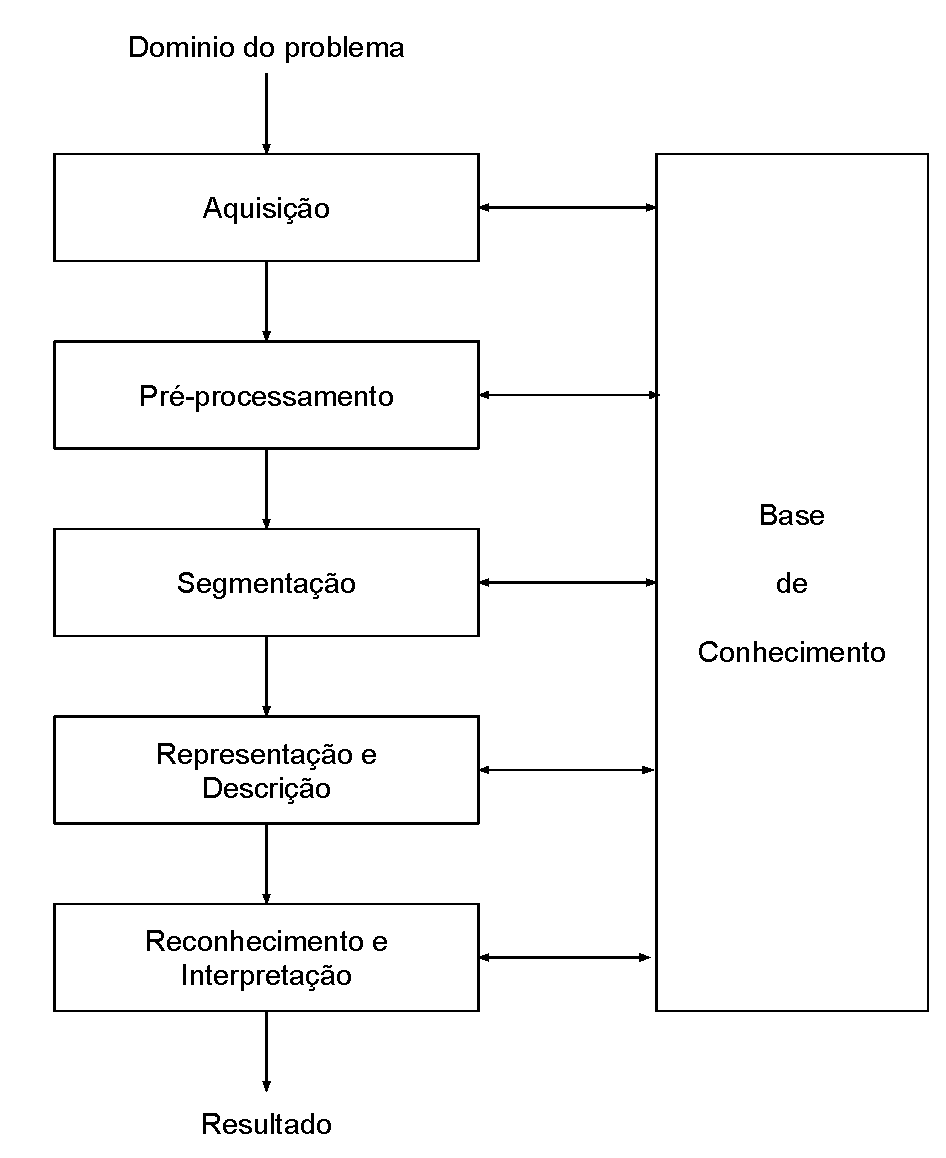
\includegraphics[width=0.6\textwidth]{imagens/PDI_Etapas_PDI.pdf}
\source{Adaptado de \citet{pedrini:2008}}
\label{fig:PDI_Etapas_PDI}
\end{figure}

A etapa de aquisição captura a imagem por meio de um dispositivo ou sensor e converte-a em uma representação adequada para o processamento digital subsequente. Os principais dispositivos para aquisição de imagens são câmeras de vídeo, tomógrafos médicos, satélites e scanners. Dentre os aspectos envolvidos nesta etapa estão a escolha do tipo de sensor, as condições de iluminação da cena, a resolução e o número de níveis de cinza ou cores da imagem digitalizada.

A imagem digital resultante do processo de aquisição pode apresentar imperfeições ou degradações decorrentes, por exemplo, das condições de iluminação ou características dos dispositivos. Segundo \citet{gonzalez:2012}, o objetivo principal das técnicas de realce é processar uma imagem, de modo que o resultado seja mais apropriado para uma aplicação específica do que a imagem original. Isso se dá por meio da aplicação de técnicas para atenuação de ruído, correção de contraste ou brilho e a suavização de determinadas propriedades da imagem.
Como a interpretação dos dados contidos em imagens digitais é uma atividade complexa, um processo intermediário de segmentação é necessário para particionar o conjunto de dados de entrada em estruturas com conteúdo semântico relevante para a aplicação em questão. Essas estruturas correspondem a objetos ou partes de objetos que auxiliarão no processo de interpretação de imagens \cite{pedrini:2008}.

Segundo \citet{gonzalez:2012}, a segmentação de imagens digitais divide uma imagem em suas partes ou objetos constituintes. O nível até o qual essa subdivisão deve ser realizada depende do problema a ser resolvido. Ou seja, a segmentação pode parar quando os objetos de interesse na aplicação tiverem sido isolados.

Em geral, a segmentação autônoma é uma das tarefas mais difíceis em processamento de imagens. Esse passo determina o eventual sucesso ou fracasso na análise. De fato, a segmentação efetiva quase sempre garante sucesso no reconhecimento. Por essa razão, um cuidado considerável deve ser tomado para melhorar as chances de uma segmentação robusta \cite{gonzalez:2012}. Ruídos na imagem podem levar os métodos de segmentação a distorcer as formas dos objetos, comprometendo seu reconhecimento, tal que regiões distintas poderiam ser incorretamente identificadas como uma única região ou, por outro lado, uma região homogênea poderia ser dividida em regiões menores \cite{pedrini:2008}.

Após a segmentação, estruturas adequadas de representação devem ser utilizadas para armazenar e manipular os objetos de interesse extraídos da imagem. O processo de descrição visa a extração de características ou propriedades que possam ser utilizadas na discriminação entre classes de objetos. Essas características são, em geral, descritas por atributos numéricos que formam um vetor de características.

A última etapa envolve o reconhecimento e a interpretação dos componentes de uma imagem. Reconhecimento ou classificação é o processo que atribui um identificador ou rótulo aos objetos da imagem, baseado nas características providas pelos seus descritores. O processo de interpretação consiste em atribuir um significado ao conjunto de objetos reconhecidos.

Nas próximas seções deste trabalho serão apresentados alguns conceitos de PDI, como histograma e convolução, que são utilizados por diversas técnicas de PDI. Ademais, serão demonstrados algoritmos de pré-processamento e segmentação de imagens que serão utilizados na proposta deste trabalho.

\section{Histograma}

Segundo \citet{pedrini:2008}, o histograma de uma imagem corresponde à distribuição dos níveis de cinza da imagem, o qual pode ser representado por um gráfico indicando o número de pixels na imagem para cada nível de cinza. Seja \(f(x,y)\) uma imagem representada por uma matriz bidimensional, com dimensões \(M\) por \(N\) pixels e contendo \(L\) níveis de cinza no intervalo \([0, L_max]\). O cálculo do histograma é apresentado no Algoritmo~\ref{alg:Histograma}. O histograma é representado por um vetor \(H\) com \(L\) elementos.

\begin{lstlisting}[caption={Cálculo do histograma de uma imagem em tons de cinza}, label=alg:Histograma, numbers=left]
// Atribuir valor zero a todos os elementos do vetor
para i = 0 ate lmax faca
    H[i] <- 0
    
// Calcular distribuicao dos niveis de cinza para cada pixel
para x = 0 ate M - 1 faca
    para y = 0 ate N - 1 faca
        H[f(x,y)] <-  H[f(x,y)] + 1
\end{lstlisting}

Na Figura~\ref{fig:PDI_Histograma} está representado (a) um exemplo de uma imagem de 64 por 64 pixels, cada um com 4 \textit{bits} de dados, permitindo 16 tonalidades de cinza. Ao lado há (b) o array \(H\) retornado pelo cálculo de histograma e (c) o gráfico representando o histograma da imagem digital.

\begin{figure}[ht]
\centering
\caption{Exemplo de uma imagem e seu histograma}
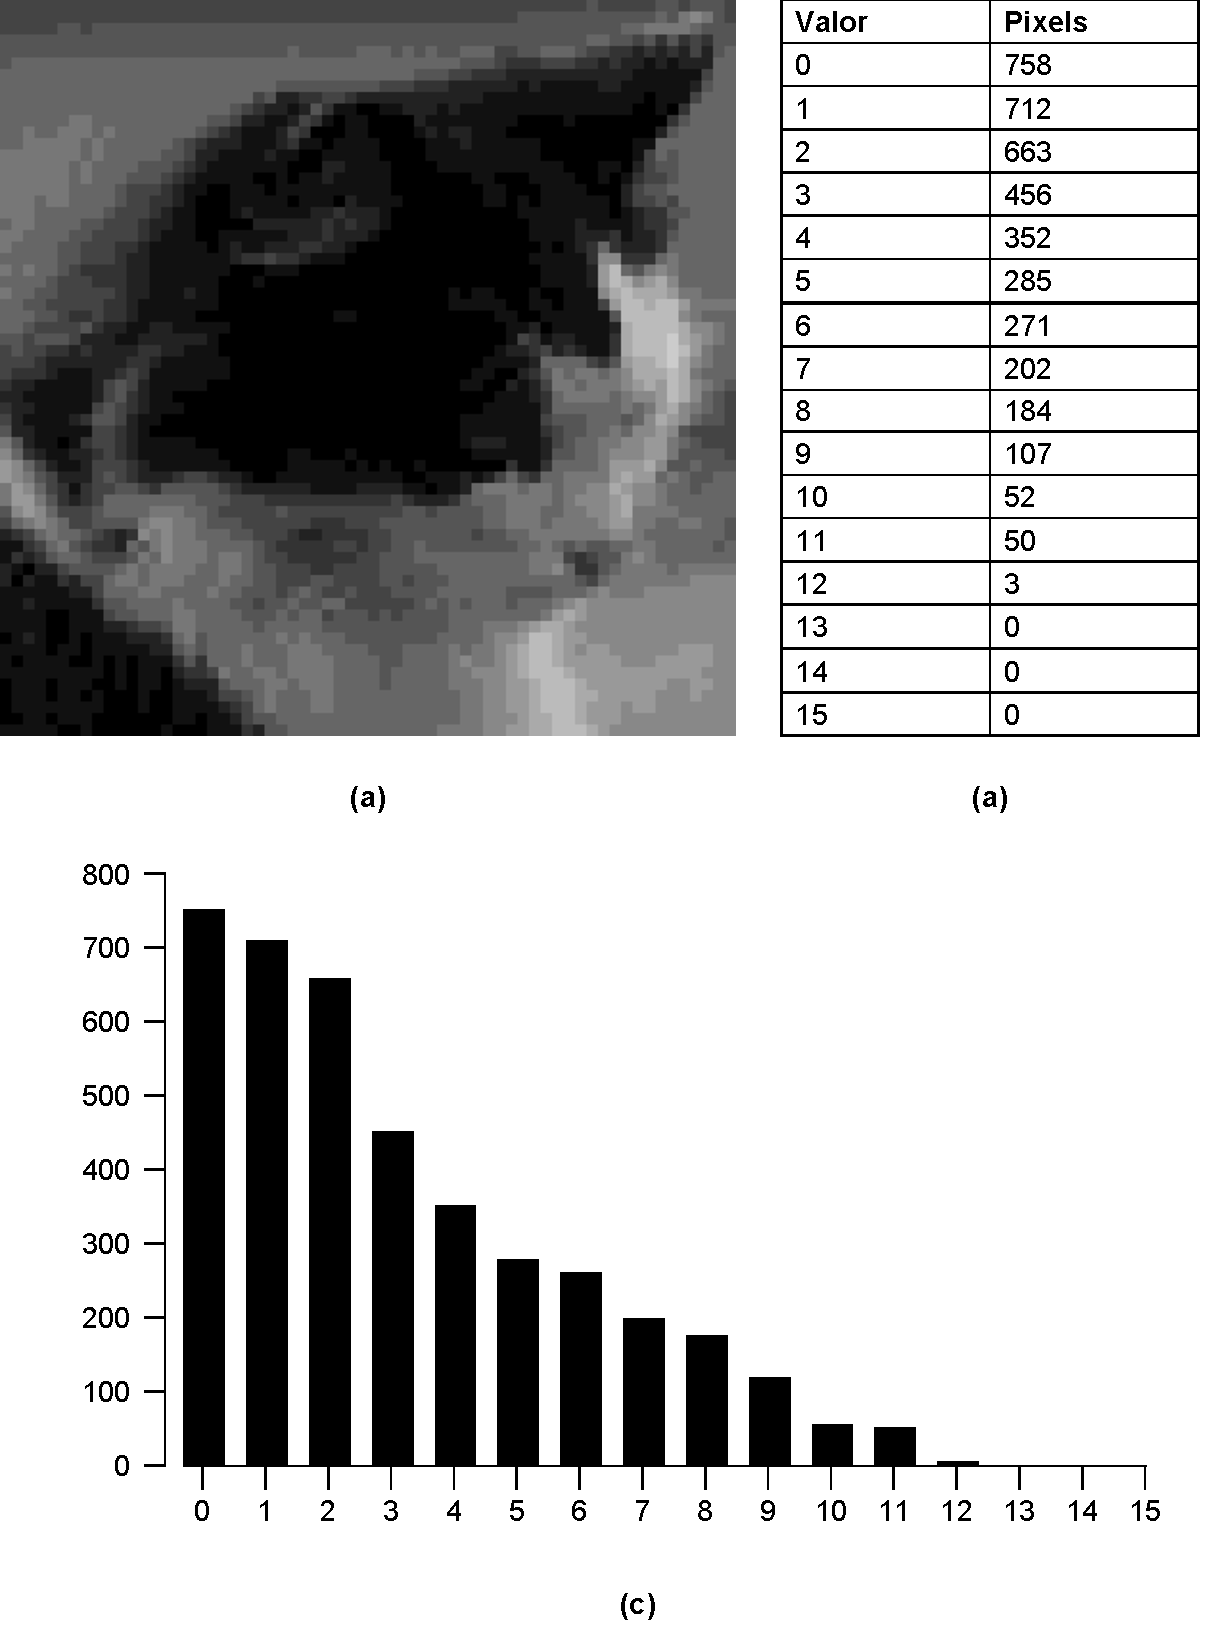
\includegraphics[width=0.5\textwidth]{imagens/PDI_Histograma.pdf}
\sourceAuthor
\label{fig:PDI_Histograma}
\end{figure}

O histograma de uma imagem fornece uma indicação de sua qualidade quanto ao nível de contraste e quanto a sua luminosidade média, ou seja, se a imagem é predominantemente clara ou escura \cite{conci:2003}. Esta relação está demonstrada na Figura~\ref{fig:PDI_Histograma_2}.

\begin{figure}[ht]
\centering
\caption{Demonstração da relação entre a imagem original e o histograma}
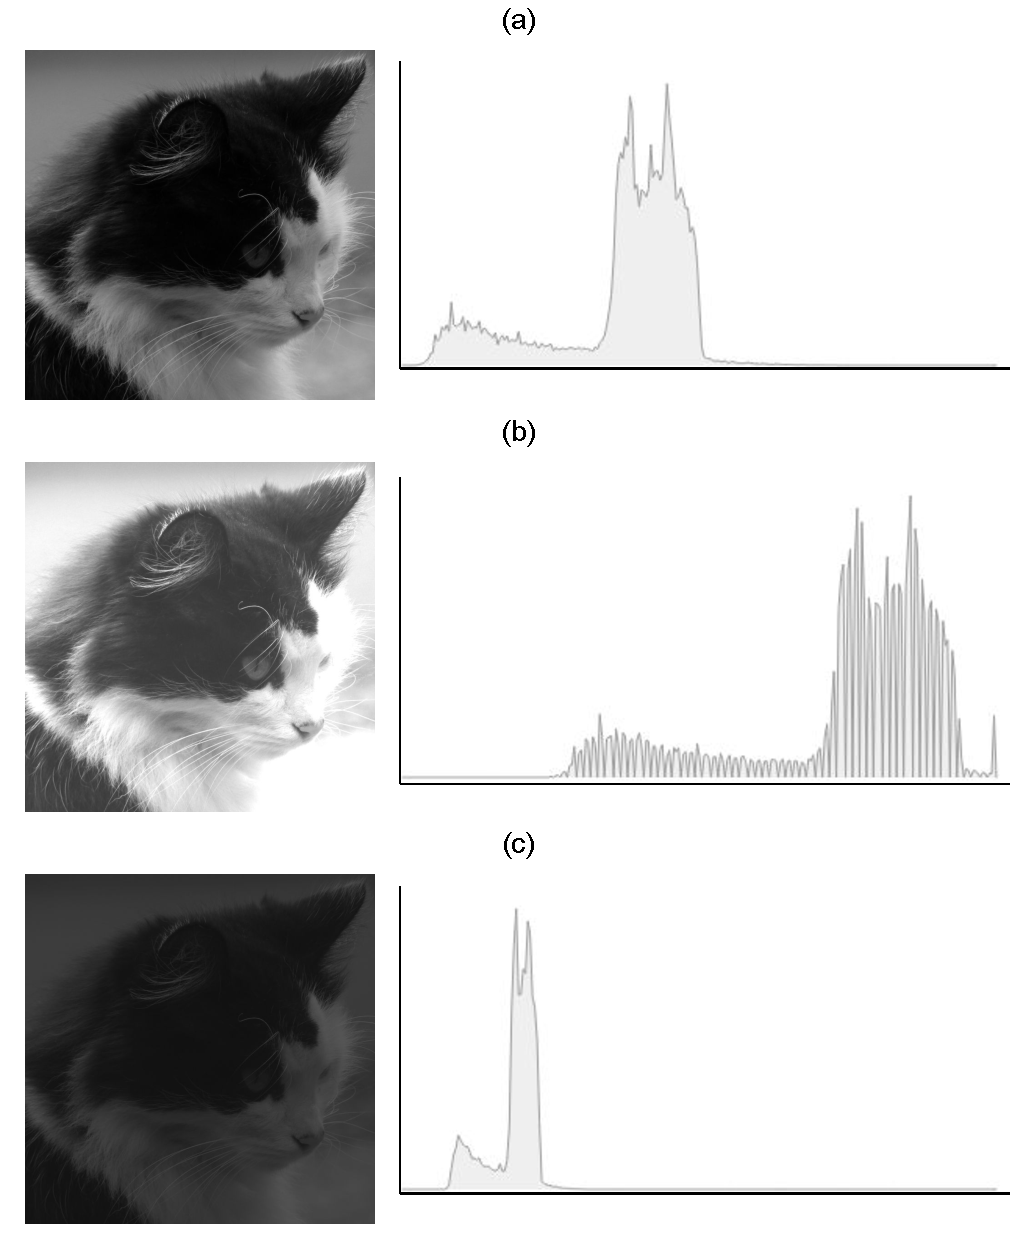
\includegraphics[width=0.6\textwidth]{imagens/PDI_Histograma_2.pdf}
\sourceAuthor
\label{fig:PDI_Histograma_2}
\end{figure}

\section{Limiarização}

Segundo \citet{pedrini:2008}, a limiarização ou thresholding é uma das técnicas mais simples de segmentação e consiste na classificação dos pixels de uma imagem de acordo com a especificação de um ou mais limiares. Cada pixel da imagem será classificado com base nos limiares definidos, de forma que a limiarização pode ser definida como \[f(x,y)=\left\{\begin{matrix} l_1, se f(x,y) \leq T_1) \\ l_2, se T_1 < f(x,y) \leq T_2)\\ l_3, se T_2 < f(x,y) \leq T_3)\\ ...\\ l_n, se f(x,y) > T_{n-1}) \end{matrix}\right.\] tal que, para cada intervalo \(T_n\), é especificado um nível de cinza correspondente \(l_n\). O algoritmo para a limiarização pode ser visto no Algoritmo~\ref{alg:Threshold}.

\begin{lstlisting}[caption={Algoritmo para limiatrização}, label=alg:Threshold, numbers=left]
para x = 0 ate M - 1 faca
    para y = 0 ate N - 1 faca
      se H[f(x,y)] < T1
         H[f(x,y)] = l1
      senao se H[f(x,y)] < T2
         H[f(x,y)] = l2
      [...]
      senao 
         H[f(x,y)] = ln
\end{lstlisting}

Quando a limiarização possui apenas um limiar ela é denominada binarização, pois a imagem resultante possui apenas dois valores de intensidade, 0 (preto) ou 1 (branco) \cite{pedrini:2008}. A forma mais comum para a identificação de um limiar adequado é a análise do histograma da imagem, visando identificar o ponto de corte entre as grandes concentrações de valores \cite{gonzalez:2012}. Um exemplo de binarização pode ser visto na Figura~\ref{fig:PDI_Limiarizacao}, demonstrando a imagem original (a), o histograma da imagem (b) e a imagem resultante da aplicação do limiar de  203 (c).

\begin{figure}[ht]
\centering
\caption{ Imagem original (a), histograma da imagem original (b) e resultado da limiarização com limiar de 203}
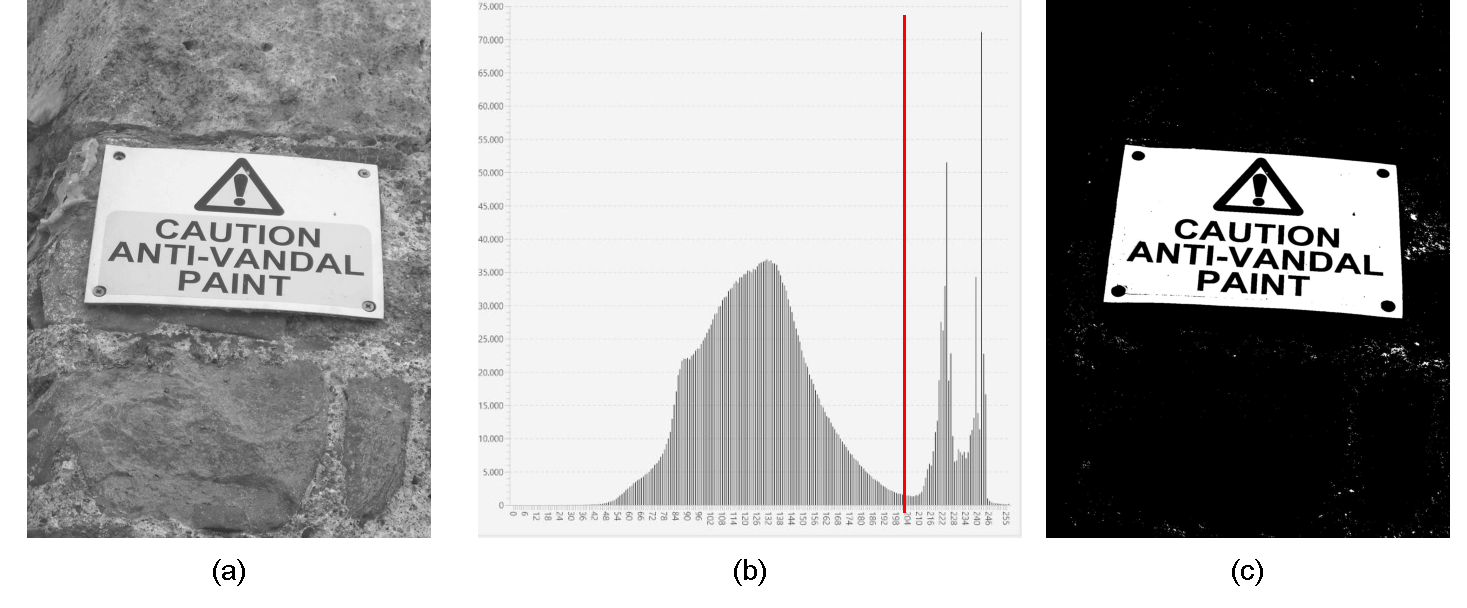
\includegraphics[width=0.9\textwidth]{imagens/PDI_Limiarizacao.pdf}
\sourceAuthor
\label{fig:PDI_Limiarizacao}
\end{figure}

A seleção correta do valor de limiar é crucial para que o processo de segmentação baseado na limiarização produza bons resultados \cite{pedrini:2008}. O resultado do uso de diferentes valores para os limiares pode ser visto na Figura~\ref{fig:PDI_Limiarizacao_2}. Na prática, espera-se que o tipo de limiarização global descrita obtenha sucesso apenas em ambientes altamente controlados \cite{gonzalez:2012}.

\begin{figure}[ht]
\centering
\caption{Demonstração de diferentes limiares. (a) 100 (b) 150 (c) 200 (d) 230}
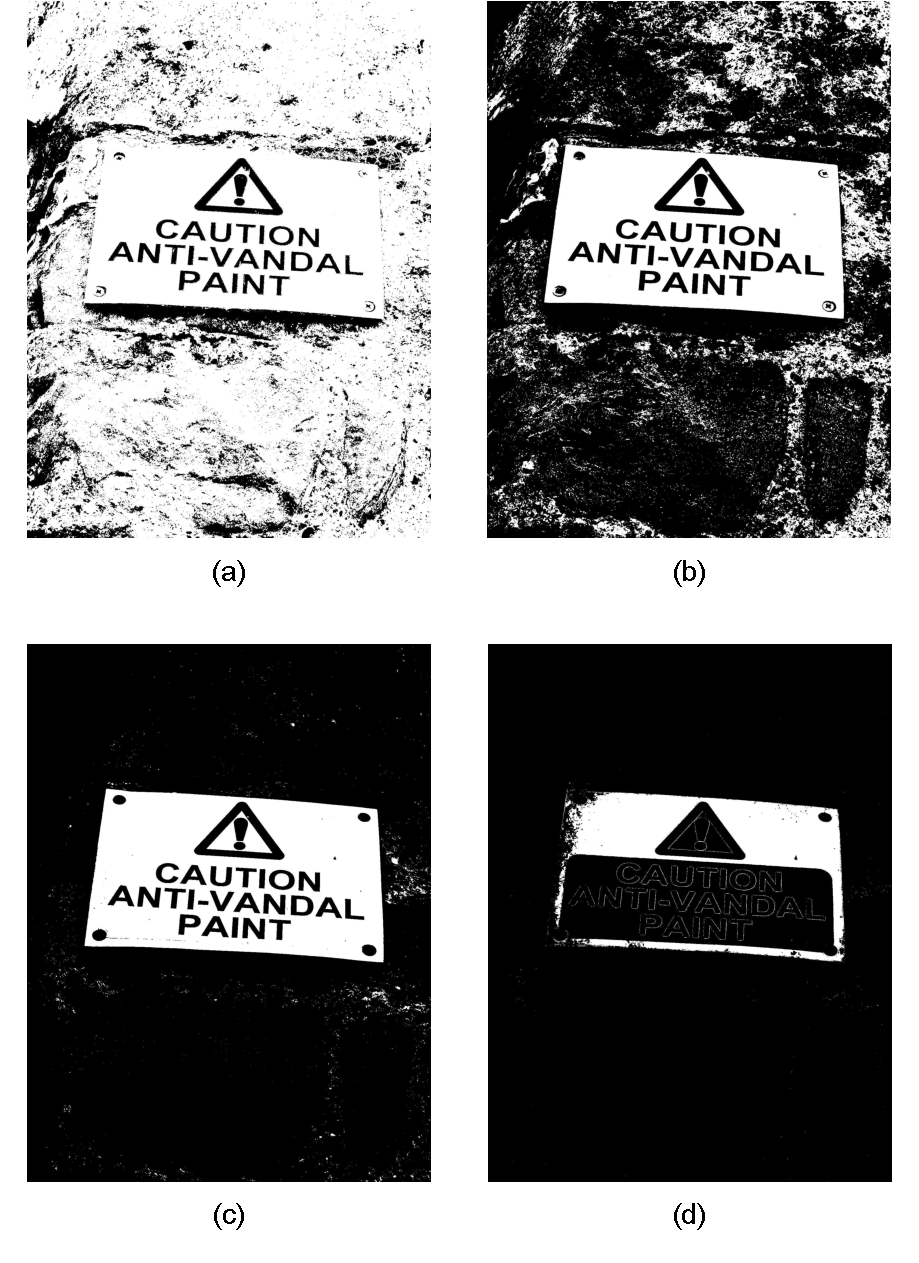
\includegraphics[width=0.4\textwidth]{imagens/PDI_Limiarizacao_2.pdf}
\sourceAuthor
\label{fig:PDI_Limiarizacao_2}
\end{figure}

\section{Brilho e contraste}

Conforme \citet{pedrini:2008}, o brilho está associado à sensação visual de intensidade luminosa ou luminância de uma fonte. Em imagens digitais o brilho é diretamente relacionado ao valor do pixel de uma imagem. Já o contraste pode ser definido como uma medida de variação relativa da luminância, ou seja, da intensidade luminosa por unidade de área.

Para realizar alterações no brilho ou contraste de um pixel da imagem, pode ser utilizada a transformação descrita pela função \(g(x,y)=a.f(x,y)+b\), tal que o parâmetro \(a\) controla a escala de níveis de cinza da imagem (contraste) e \(b\) ajusta seu brilho \cite{pedrini:2008}. O valor de \(f(x,y)\) é o valor atual do pixel na posição calculada e o valor de \(g(x,y)\) é o valor do pixel na nova imagem. Na Figura~\ref{fig:PDI_Brilho_e_Contraste} é possível ver a diferença causada pela aplicação da função com diferentes parâmetros para \(a\) e \(b\) \cite{pedrini:2008}. O algoritmo para aplicação do brilho e contraste pode ser vista no Algoritmo~\ref{alg:Brilho_Contraste}

\begin{lstlisting}[caption={Algoritmo para aplicação de brilho e contraste}, label=alg:Brilho_Contraste, numbers=left]
para x = 0 ate M - 1 faca
    para y = 0 ate N - 1 faca
      H[f(x,y)] = a * H[f(x,y)] + b
\end{lstlisting}

\begin{figure}[ht]
\centering
\caption{a) Imagem original; b) Imagem transformada com a=1 e b=100; c) Imagem com a=1 e b=-100; d) Imagem transformada com a=1.5 e b=0; e) Imagem transformada com a=0.5 e b=0; f) Imagem transformada com a=1.4 e b=50}
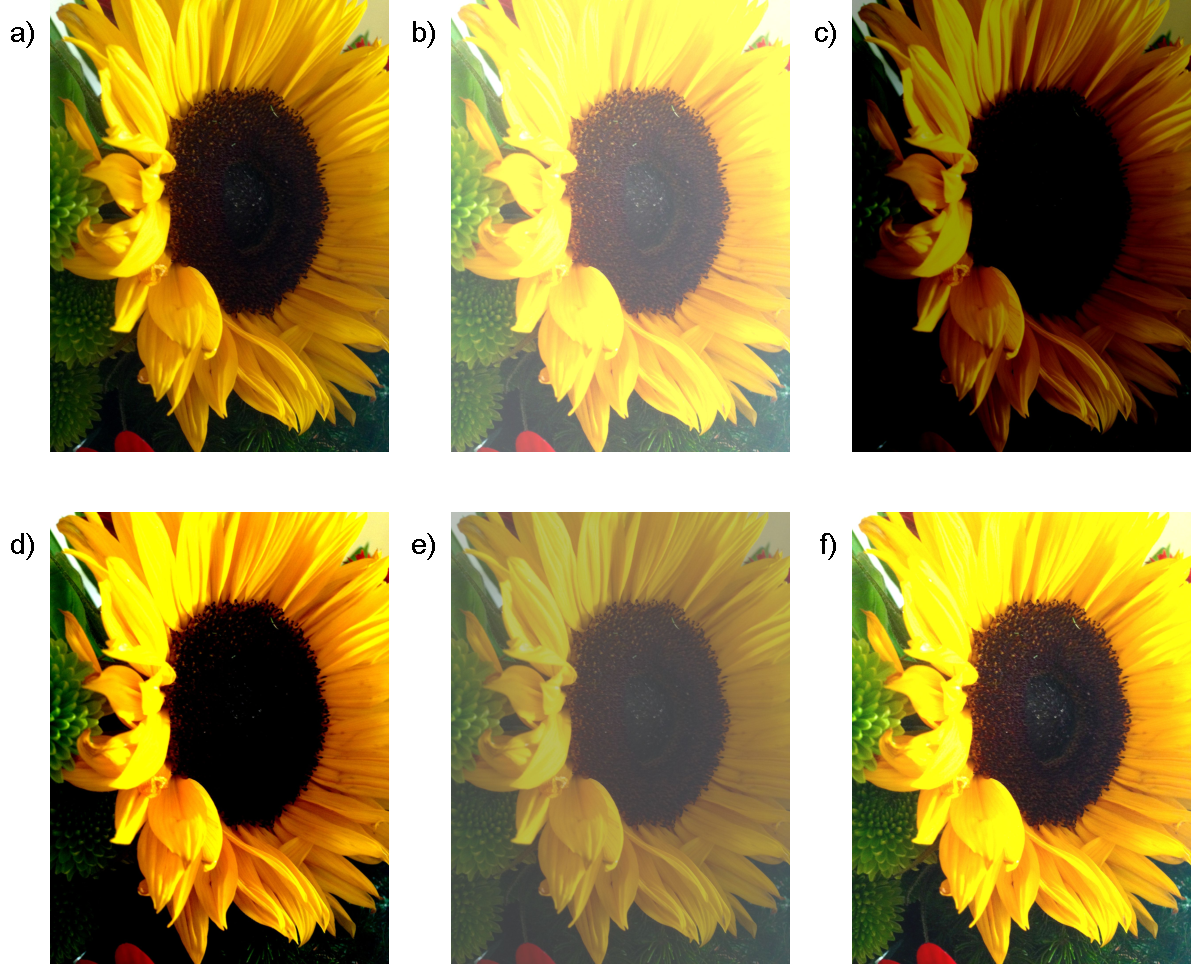
\includegraphics[width=0.5\textwidth]{imagens/PDI_Brilho_e_Contraste.pdf}
\sourceAuthor
\label{fig:PDI_Brilho_e_Contraste}
\end{figure}

Outra função linear comum é a transformação inversa, que produz o negativo de uma imagem. Nessa transformação, a intensidade da imagem de saída diminui à medida que a intensidade da imagem de entrada aumenta \cite{pedrini:2008}. Ela pode ser representada com a função de transformação linear demonstrada acima utilizando os parâmetros \(a=-1\) e \(b=f_{max}\), sendo \(f_{max}\) o valor máximo do pixel. Um exemplo de inversão de imagens pode ser vista na Figura~\ref{fig:PDI_Inversao}.

\begin{figure}[ht]
\centering
\caption{Demonstração de inversão. a) Imagem original; b) Imagem invertida}
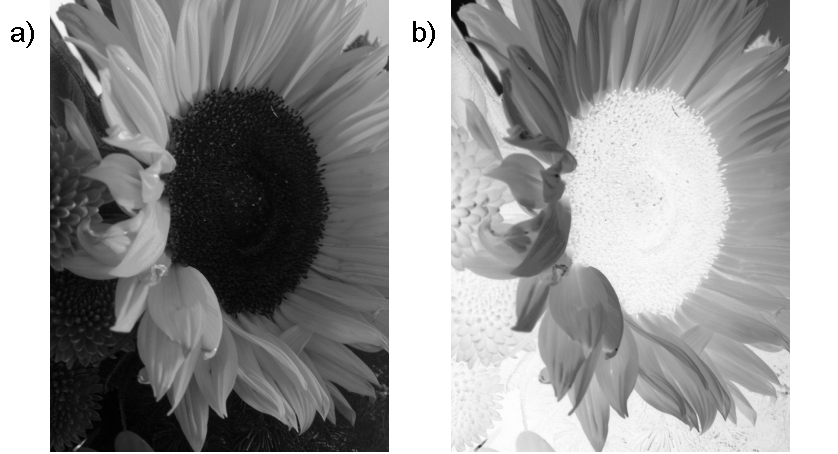
\includegraphics[width=0.5\textwidth]{imagens/PDI_Inversao.pdf}
\sourceAuthor
\label{fig:PDI_Inversao}
\end{figure}

\section{Morfologia Matemática}

Segundo \citet{pedrini:2008} a morfologia matemática consiste em uma metodologia para análise de imagens que permite a construção de operadores úteis para a descrição de objetos em imagens. Ela foi originalmente desenvolvida para manipular imagens binárias, sendo posteriormente estendida para tratar imagens em níveis de cinza.

A morfologia matemática utiliza a teoria de conjuntos para representar a forma dos objetos em uma imagem. Por convenção, objetos em uma imagem binária serão representados por pixels com valor 1 enquanto o fundo será formado por pixels com valor 0. Dessa forma, é possível representar uma imagem binária como uma coleção de coordenadas discretas que correspondem aos pontos que fazem parte dos objetos da imagem, o que pode ser visualizado na Figura~\ref{fig:PDI_Conjunto}.

\begin{figure}[ht]
\centering
\caption{Demonstração do conjunto (b) que representa a imagem binária (a)}
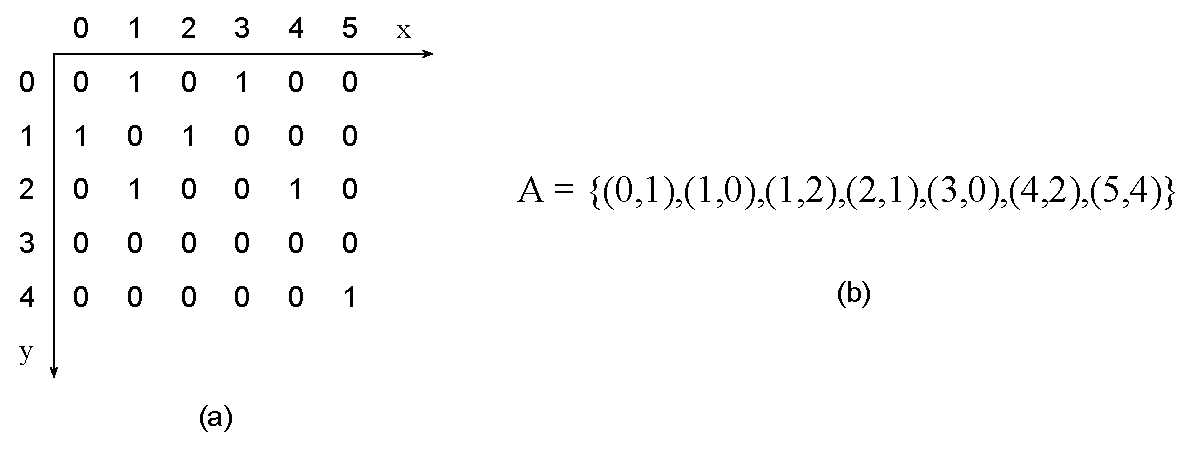
\includegraphics[width=0.8\textwidth]{imagens/PDI_Conjunto.pdf}
\source{adaptado de \citet{pedrini:2008}, pg. 328}
\label{fig:PDI_Conjunto}
\end{figure}

Um operador morfológico é um mapeamento entre o conjunto A que define a imagem e um conjunto B, chamado de elemento estruturante. O elemento estruturante é expresso com respeito a uma origem local \cite{pedrini:2008}.

\subsection{Dilatação e Erosão}

A operação de dilatação entre o conjunto A e um elemento estruturante B é definida como a adição de \citet{minkowski:1911}, ou seja: \[D(A,B)=A\oplus B=\bigcup_{b\in B}^{ } (A+b)\]

De acordo com esta equação, o processo de dilatação entre \(A\) e \(B\) corresponde ao conjunto de todas as translações de B com os pontos da imagem em que há pelo menos um elemento não nulo (com valor 1) em comum com o conjunto \(A\) \cite{pedrini:2008}. 

Na Figura~\ref{fig:PDI_Dilatacao_1} está demonstrado a aplicação da dilatação em uma imagem de entrada (a) utilizando o elemento estruturante (b). A origem do elemento estruturante está indicada por uma cruz. Em (c) é possível ver o elemento estruturante sendo aplicado sobre o pixel da posição (3, 4). Na dilatação, caso a origem do elemento estruturante seja não nula, todos os pixels vizinhos receberão o valor do elemento estruturante. A imagem final está demonstrada em (d).

\begin{figure}[ht]
\centering
\caption{Demonstração do processo de dilatação}
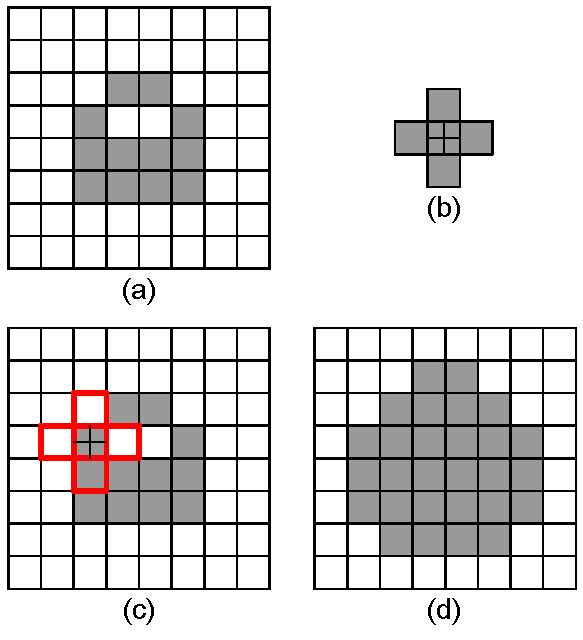
\includegraphics[width=0.5\textwidth]{imagens/PDI_Dilatacao_1.pdf}
\sourceAuthor
\label{fig:PDI_Dilatacao_1}
\end{figure}

O resultado do processo de dilatação é dependente do elemento estruturante utilizado. Na Figura~\ref{fig:PDI_Dilatacao_2} é possível ver o efeito de dois elementos estruturantes diferentes sendo aplicados sobre a mesma imagem de origem da Figura~\ref{fig:PDI_Dilatacao_1} (a).

\begin{figure}[ht]
\centering
\caption{Elementos estruturantes na dilatação}
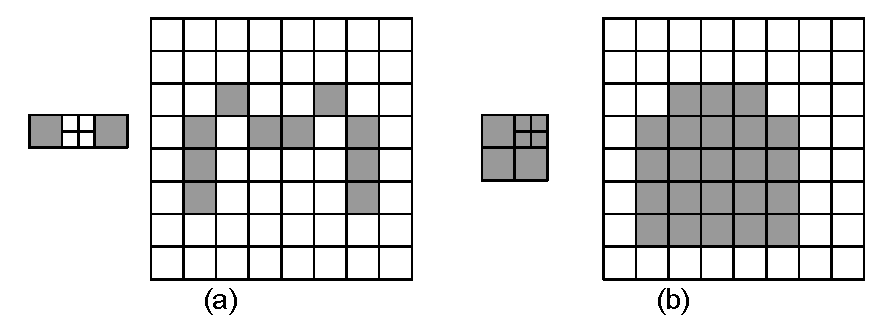
\includegraphics[width=0.8\textwidth]{imagens/PDI_Dilatacao_2.pdf}
\sourceAuthor
\label{fig:PDI_Dilatacao_2}
\end{figure}

A operação de erosão entre o conjunto A e o elemento estruturante B é definida como a subtração de \citet{minkowski:1911}, ou seja \[\varepsilon(A,B)=A\ominus B=\bigcap_{b\in B}^{ } (A-b)\]

De acordo com esta equação, o resultado da erosão pode ser calculado como o conjunto de pixels, tal que o elemento estruturante \(B\), transladado com respeito a cada um dos pixels dos objetos na imagem \(A\), corresponde ao conjunto de pixels dos objetos em A. Assim, os pixels que não correspondem ao padrão definido pelo elemento estruturante não pertencerão ao resultado. O processo de erosão está descrito na Figura~\ref{fig:PDI_Erosao_1}.

\begin{figure}[ht]
\centering
\caption{Demonstração do processo de erosão}
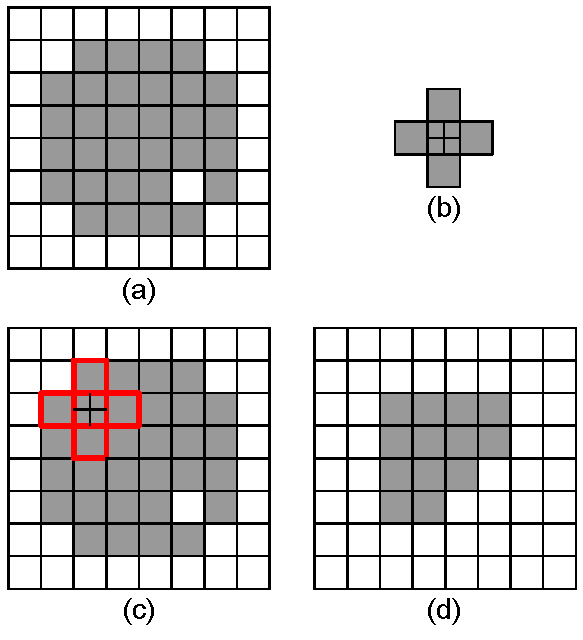
\includegraphics[width=0.5\textwidth]{imagens/PDI_Erosao_1.pdf}
\sourceAuthor
\label{fig:PDI_Erosao_1}
\end{figure}

\subsection{Abertura e Fechamento}

Duas outras operações morfológicas importantes em análise de imagens são a abertura e o fechamento. A abertura de A por B é definida como \(A \circ  B = (A \ominus B) \oplus A\) \cite{pedrini:2008}. Isso significa que a abertura é a erosão de A por B, seguida da dilatação da imagem resultante por A.

O fechamento de A por B é definido como \(A \bullet  B = (A \oplus B) \ominus A\) \cite{pedrini:2008}. Ou seja, é realizada a dilatação de A por B, seguida da erosão da imagem resultante por B.
Na Figura~\ref{fig:PDI_Abertura_Fechamento_1} é possível visualizar o efeito dos processos de fechamento (a) e abertura (a) em uma imagem binária utilizanod um elemento estruturante de vizinhança-8.

\begin{figure}[ht]
\centering
\caption{Demonstração de abertura e fechamento}
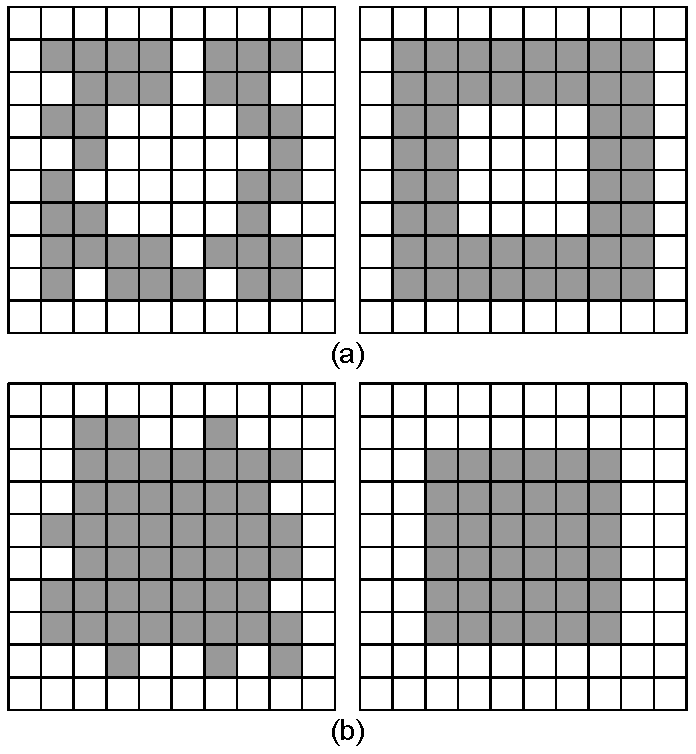
\includegraphics[width=0.5\textwidth]{imagens/PDI_Abertura_Fechamento_1.pdf}
\sourceAuthor
\label{fig:PDI_Abertura_Fechamento_1}
\end{figure}

\section{Filtragem da Imagem}

Conforme \citet{conci:2003}, o uso de filtros em imagens objetiva melhorar a qualidade das imagens através da amplificação do seu contraste, eliminação de padrões periódicos ou aleatórios (como ruídos ou imperfeições das imagens), melhoria no seu foco e acentuação de características. Os filtros podem ser classificados como passa-baixa e passa-alta.
	
Para a aplicação de filtros em imagens pode ser utilizado um processo denominado convolução. Conforme \cite{pedrini:2008}, a convolução é um processo que envolve a aplicação de uma máscara quadrada \(w\) de tamanho \(n\) por \(n\). Cada posição da máscara possui um valor numérico denominado peso ou coeficiente. Cada pixel \(f(x,y)\) da imagem é substituído por um novo valor, que depende do valor dos pixels vizinhos e dos pesos da máscara. Os coeficientes da máscara são multiplicados pela intensidade dos vizinhos correspondentes e então somados, resultando no valor do pixel central.

Denotando os níveis de cinza da imagem sob a máscara por \(z_i=f(x,y)\), \(1\leq i\leq 9\), a resposta da máscara é \(R=w_1.z_1+w_2.z_2+...+w_9z_9 = \sum_{i=1}^{9}w_i.z_i\) em que \(w_i\) representa os coeficientes das máscaras. Um exemplo de aplicação de convolução pode ser visualizado na Figura~\ref{fig:PDI_Convolucao}, onde (a) representa a máscara \(w\) e (b) representa a imagem de origem. Em (c), (d) e (e) representam os passos da convolução para o pixel (2, 2).
	
\begin{figure}[ht]
\centering
\caption{Exemplo do processo de convolução}
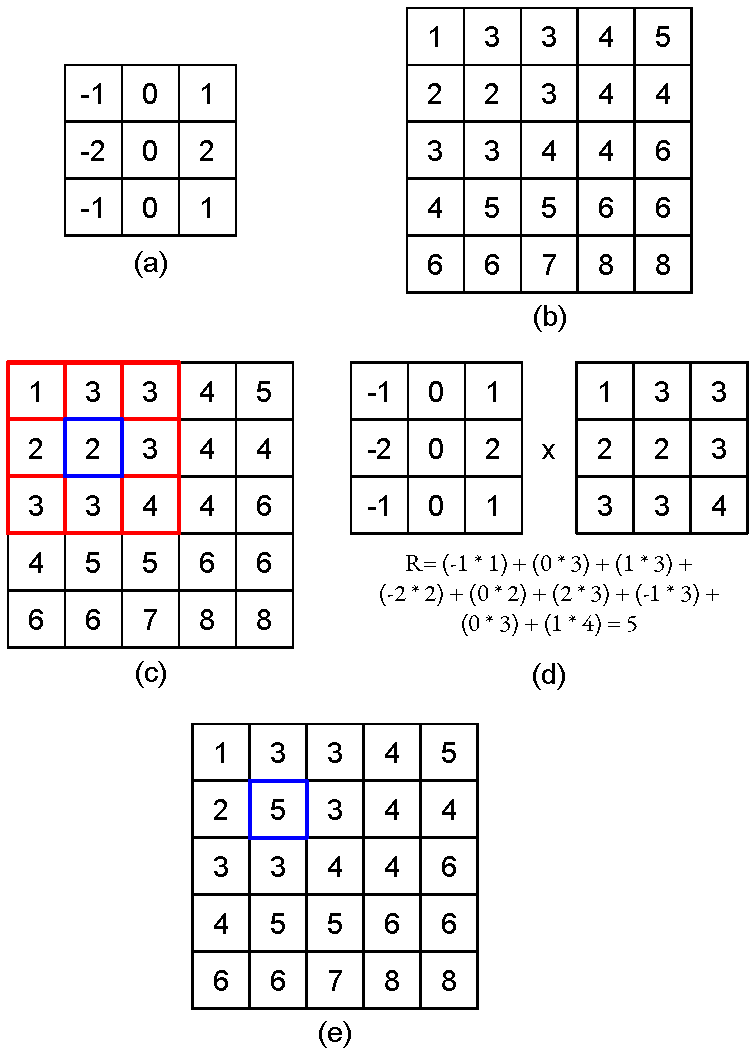
\includegraphics[width=0.5\textwidth]{imagens/PDI_Convolucao.pdf}
\sourceAuthor
\label{fig:PDI_Convolucao}
\end{figure}

\subsection{Filtros passa-baixas}

São denominados filtros passa-baixas aqueles que atenuam ou eliminam os componentes de alta-frequência enquanto deixam as frequências baixas inalteradas. Os componentes de alta-frequência caracterizam bordas e outros detalhes finos de uma imagem, de forma que o efeito resultante da filtragem passa-baixas é o borramento da imagem \cite{gonzalez:2012}. Existem diversos filtros de classe passa-baixas, porém, neste trabalho, serão apresentados apenas os mais utilizados.

\subsubsection{Filtro da Média e Mediana}

Um dos filtros passa-baixa mais simples é o filtro da média, em que cada pixel é substituído pelo valor médio de seus vizinhos. O filtro da média é um filtro passa-baixa utilizado para fins de suavização de imagens \cite{pedrini:2008}. Na Figura~\ref{fig:PDI_Mascara_Media} estão representadas máscaras de filtro da média de tamanho 3x3 e 5x5, respectivamente.

\begin{figure}[ht]
\centering
\caption{Exemplo de máscaras de convoulção de média}
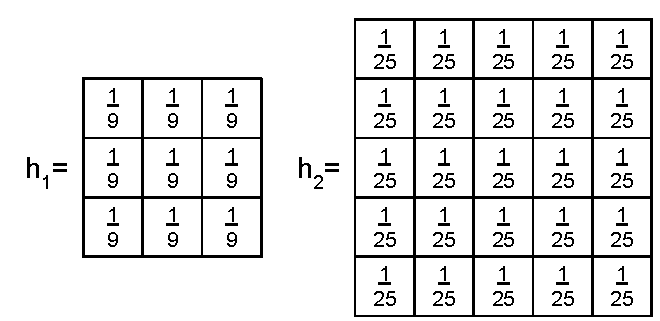
\includegraphics[width=0.5\textwidth]{imagens/PDI_Mascara_Media.pdf}
\source{adaptado de \citet{pedrini:2008}, pg. 328}
\label{fig:PDI_Mascara_Media}
\end{figure}

O filtro de média é considerado um filtro linear, pois ele efetua a suavização homogênea de detalhes finos e bordas da imagem, causando uma perda de detalhes. Existe outra classe de filtros denominada filtros não-lineares que procura evitar esta perda \cite{pedrini:2008}.

Um filtro não-linear bastante empregado no processamento digital de imagem é o filtro de mediana, que consiste em substituir a intensidade de cada pixel pela mediana das intensidades na vizinhança do pixel. O filtro de mediana não utiliza a convolução, mas sim ordena a intensidade da vizinhança e utiliza a intensidade do pixel que estiver na posição central. Para uma vizinhança de \(n\)x\(n\) pixels, sendo \(n\) ímpar, a mediana das intensidades ordenada encontra-se na posição \(\frac{n^2+1}{2}\). Caso \(n\) seja par, é necessário realizar a média aritmética dos dois elementos mais próximos ao centro \cite{gonzalez:2012}. 

Seus resultados são geralmente melhores que o filtro da média. Isso ocorre devido ao fato de que, se existe um ruído entre os elementos da máscara, este valor estará presente nas primeiras ou últimas posições da vizinhança ordenada. Assim, valores de intensidade discrepantes serão completamente desconsiderados, ao invés de impactar no valor da intensidade \cite{conci:2003}. Na Figura~\ref{fig:PDI_Media_Mediana} é possível ver a comparação entre os filtros de média (b) e mediana (c) para a remoção do ruído de tipo sal e pimenta da imagem original (a).

\begin{figure}[ht]
\centering
\caption{ Demonstração dos filtros de média e mediana}
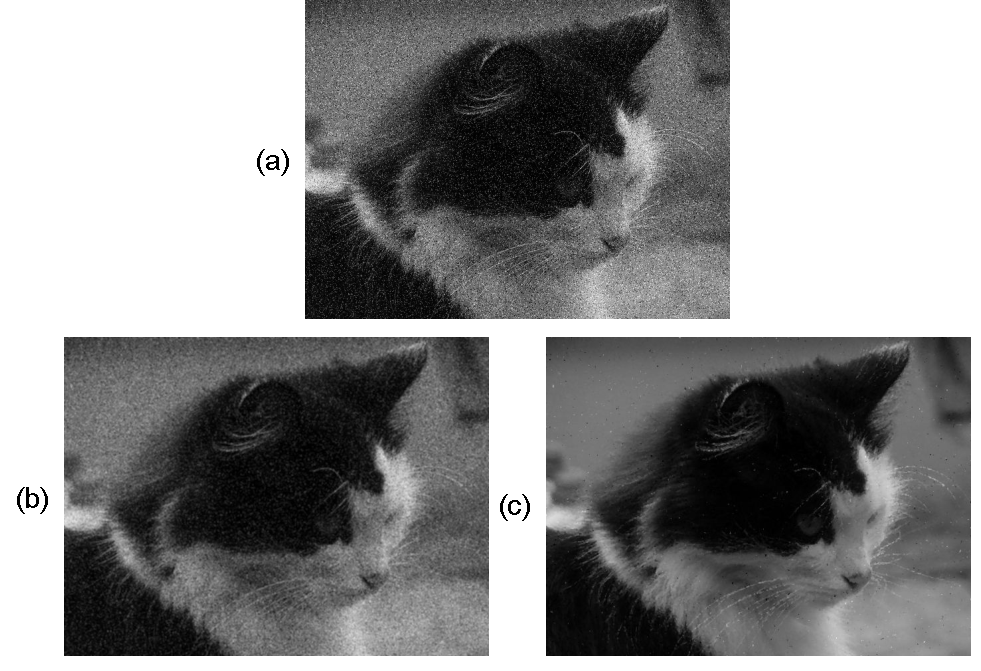
\includegraphics[width=0.6\textwidth]{imagens/PDI_Media_Mediana.pdf}
\sourceAuthor
\label{fig:PDI_Media_Mediana}
\end{figure}

\subsubsection{Filtro Gaussiano}

Segundo \citet{conci:2003}, o filtro de Gauss ou Gaussiano é o filtro linear passa-baixa mais importante. Assim como outros filtros dessa classe, é utilizado para reduzir a quantidade de variação de intensidade entre um pixel e seus vizinhos, efetuando a redução de ruídos e outras trocas bruscas de frequência da imagem. Na Figura~\ref{fig:PDI_Gauss} é possível ver a aplicação do filtro Gaussiano em uma imagem (a) com máscaras de tamanho 3x3 (b) e 5x5 (c).

\begin{figure}[ht]
\centering
\caption{Demonstração do Filtro de Gauss}
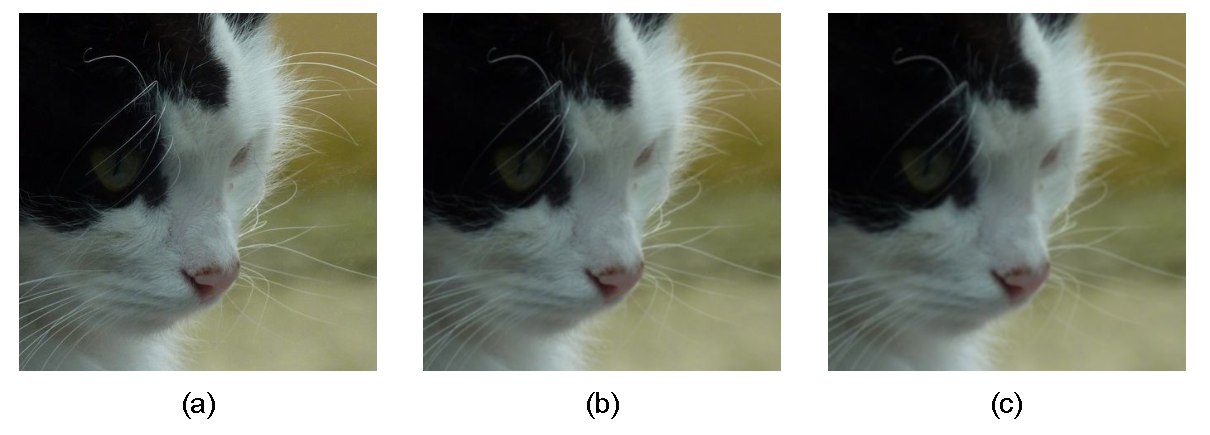
\includegraphics[width=0.7\textwidth]{imagens/PDI_Gauss.pdf}
\sourceAuthor
\label{fig:PDI_Gauss}
\end{figure}

Segundo \citet{pedrini:2008}, os coeficientes da máscara de processamento do filtro Gaussiano são obtidos através de uma função Gaussiana bidimensional. A função Gaussiana com média zero e desvio padrão \(\sigma\) é descrita por \[G(x,y)=\frac{1}{2\pi\sigma\theta^2} e^{\frac{-(x^2+y^2)}{2\sigma^2}  }\]

A aplicação do filtro Gaussiano é feita com operações de convolução, então é necessário transformar a função gaussiana em estrutura de uma máscara. O tamanho da máscara que descreve o filtro de Gauss é muito grande, mas é possível descartar os valores que estão além de três posições do centro \cite{conci:2003}. Duas máscaras desse filtro estão exemplificadas abaixo, ambas com desvio-padrão igual a 1.

\[Z=\frac{1}{256}\begin{bmatrix}
1 & 4 & 6 & 5 & 1\\ 
4 & 16 & 24 & 16 & 4\\ 
6 & 24 & 36 & 24 & 6\\ 
4 & 16 & 24 & 16 & 4\\ 
1 & 4 & 6 & 4 & 1
\end{bmatrix}
\; \; \; \; \; \; 
Z=\frac{1}{16}\begin{bmatrix}
1 & 2 & 1\\ 
2 & 4 & 2\\ 
1 & 2 & 1
\end{bmatrix}
\]

\subsection{Filtros passa-altas}

Os filtros passa-altas atenuam ou eliminam os componentes de baixa-frequência, mantendo frequências altas. Como as baixas frequências são responsáveis pelas características que variam lentamente em uma imagem, como o contraste total e a intensidade média, o efeito resultante da filtragem passa-altas é uma redução destas características, correspondente a uma aparente agudização de bordas, trocas repentinas de intensidade e também ruídos \cite{gonzalez:2012}. Existem inúmeros filtros do tipo passa-alta, alguns destes sendo apresentados neste trabalho.

\subsubsection{Operador de Sobel}

O operador de Sobel foi proposto por \citet{sobel:1968}. Ele é composto por duas máscaras que aproximam a magnitude do gradiente com as diferenças dos níveis de cinza da imagem. Os dois gradientes representam, respectivamente, as variações de intensidade no eixo horizontal (\(G_x\)) e vertical (\(G_y\)). Ao efetuar operações de convolução dessas máscaras com a imagem, as variações de intensidade dos níveis de cinza em cada eixo são detectadas. O resultado final da convolução é dado por \(\sqrt[]{{G_x}^2 + {G_y}^2}\). Este valor resultante deve então ser aplicado a um limiar, identificando se o ponto é ou não a borda \cite{pedrini:2008}. Um exemplo da aplicação de Sobel pode ser visto na Figura~\ref{fig:PDI_Sobel} com um limiar de 40.

\begin{table}
\centering
\caption{Máscaras do operador de Sobel}
\label{tab:Sobel}
\begin{tabular}{lllllll}
\cline{1-3} \cline{5-7}
\multicolumn{1}{|l|}{-1} & \multicolumn{1}{l|}{0} & \multicolumn{1}{l|}{1} & \multicolumn{1}{l|}{} & \multicolumn{1}{l|}{-1} & \multicolumn{1}{l|}{-2} & \multicolumn{1}{l|}{-1} \\ \cline{1-3} \cline{5-7} 
\multicolumn{1}{|l|}{-2} & \multicolumn{1}{l|}{0} & \multicolumn{1}{l|}{2} & \multicolumn{1}{l|}{} & \multicolumn{1}{l|}{0}  & \multicolumn{1}{l|}{0}  & \multicolumn{1}{l|}{0}  \\ \cline{1-3} \cline{5-7} 
\multicolumn{1}{|l|}{-1} & \multicolumn{1}{l|}{0} & \multicolumn{1}{l|}{1} & \multicolumn{1}{l|}{} & \multicolumn{1}{l|}{1}  & \multicolumn{1}{l|}{2}  & \multicolumn{1}{l|}{1}  \\ \cline{1-3} \cline{5-7} 
                         & \(G_x\)                   &                        &                       &                         & \(G_y\)                    &                        
\end{tabular}
\end{table}

\begin{figure}[ht]
\centering
\caption{Demonstração do Filtro de Sobel}
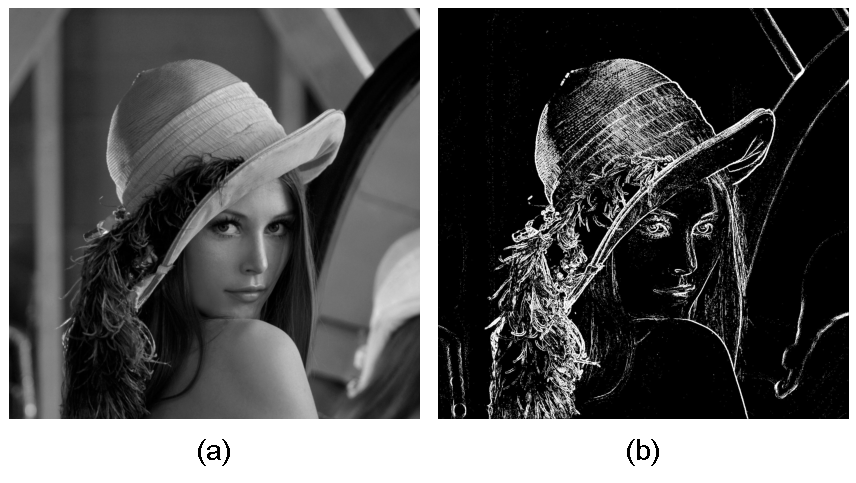
\includegraphics[width=0.6\textwidth]{imagens/PDI_Sobel.pdf}
\sourceAuthor
\label{fig:PDI_Sobel}
\end{figure}

\subsubsection{Operador de Canny}

O detector de bordas de Canny é mais complexo, mas geralmente superior aos demais métodos passa-alta \cite{gonzalez:2012}. Ele foi proposto por \citet{canny:1987} e é composto por 4 etapas básicas: suavização da imagem de entrada com a aplicação do filtro gaussiano; cálculo da magnitude do gradiente e ângulos das imagens; identificação dos pontos de máxima ou mínima intensidade de acordo com o gradiente; e, por fim, é definido o limiar e feita a análise de conectividade dos pixels classificados como borda \cite{gonzalez:2012}. Um exemplo do operador de Canny com limiar de 25 pode ser visto na Figura~\ref{fig:PDI_Canny}.

\begin{figure}[ht]
\centering
\caption{Demonstração do Filtro de Canny}
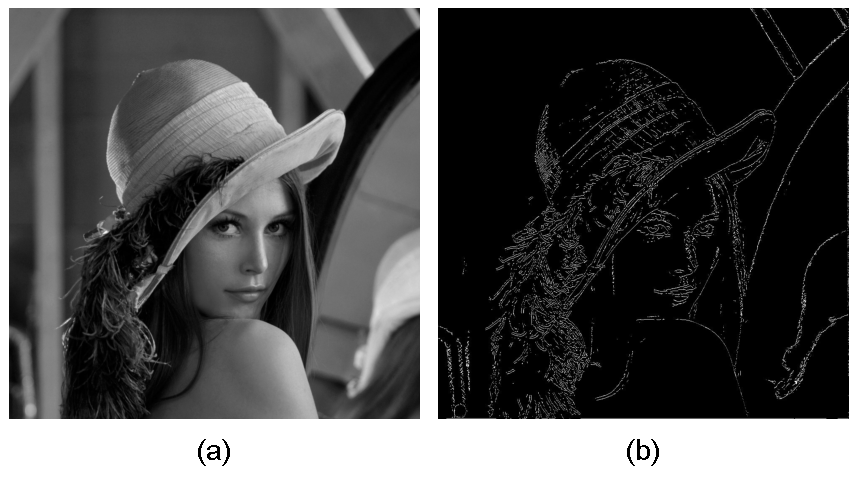
\includegraphics[width=0.6\textwidth]{imagens/PDI_Canny.pdf}
\sourceAuthor
\label{fig:PDI_Canny}
\end{figure}

% TODO: Marta: Complementar aqui dizendo como fazer isso

\section{Transformações Geométricas}

Conforme \citet{conci:2003} as transformações geométricas são operações realizadas em imagens digitais que movem os pixels da imagem de origem entre uma posição \((x_o,y_o)\) para a posição \((x_d,y_d)\) da imagem de destino, ou seja, modificam a posição dos pixels no espaço de imagem. As principais transformações geométricas são: translação, mudança de escala, rotação e espelhamento.

Para realizar a conversão de coordenadas é utilizado um sistema de coordenadas homogêneo, ou seja, de dimensão \(n+1\). No caso de imagens bidimensionais, é acrescentada a terceira coordenada \(w\) com o valor 1 aos pontos \((x, y)\). Com o sistema de coordenadas homogêneas, todas as transformações geométricas principais são tratadas através de multiplicação de matrizes.

\subsection{Translação}

Transladar um objeto significa deslocar, mover ou somar a cada um de seus pontos \((x_o,y_o)\) uma quantidade \((T_x,T_y)\). A translação 2D na forma matricial em coordenadas homogêneas é definida pela equação

\[
\begin{bmatrix}
x_d\\ 
y_d\\ 
1
\end{bmatrix}
=
\begin{bmatrix}
1 & 0 & T_x\\ 
0 & 1 & T_y\\ 
0 & 0 & 1
\end{bmatrix}
\begin{bmatrix}
x_o\\ 
y_o\\ 
1
\end{bmatrix}
\]

\subsection{Escala}

A mudança de escala significa variar o seu tamanho, de forma semelhante a um \textit{zoom in} ou \textit{zoom out}. A operação básica consiste em multiplicar cada um de seus pontos \((x_o,y_o)\) por um fator escalar \((S_x,S_y)\). A escala 2D na forma matricial em coordenadas homogêneas é definida pela equação

\[
\begin{bmatrix}
x_d\\ 
y_d\\ 
1
\end{bmatrix}
=
\begin{bmatrix}
S_x & 0 & 0\\ 
0 & S_y & 0\\ 
0 & 0 & 1
\end{bmatrix}
\begin{bmatrix}
x_o\\ 
y_o\\ 
1
\end{bmatrix}
\]

O fato de os valores de x e y serem inteiros (pois representam as coordenadas da imagem) pode gerar problemas. Considerando, por exemplo, um escalar de \((2,2)\). O pixel da posição \((1,1)\) irá virar \((2,2)\), enquanto o pixel da posição \((2,2)\) irá virar \((4,4)\). Isso deixará o pixel \((3,3)\) sem valor de origem. Isso pode ser corrigido realizando uma interpolação linear ou bilinear entre os pontos existentes.

\subsection{Rotação}

A rotação utilizando um ângulo  relativo à origem consiste em encontrar, para cada pixel \((x_o,y_o)\) um outro pixel \((x_d,y_d)\) sobre uma circunferência centrada na origem que passa pelos dois pontos com ângulo \(\theta=p \hat{o} q\). 

A rotação da imagem sobre o eixo Z na forma matricial em coordenadas homogêneas é definida pela equação

\[
\begin{bmatrix}
x_d\\ 
y_d\\ 
1
\end{bmatrix}
=
\begin{bmatrix}
\cos{\theta} & -\sin{\theta} & 0\\ 
\sin{\theta} & \cos{\theta} & 0\\ 
0 & 0 & 1
\end{bmatrix}
\begin{bmatrix}
x_o\\ 
y_o\\ 
1
\end{bmatrix}
\]

A rotação da imagem sobre o eixo X na forma matricial em coordenadas homogêneas é definida pela equação
\[
\begin{bmatrix}
x_d\\ 
y_d\\ 
1
\end{bmatrix}
=
\begin{bmatrix}
1 & 0 & 0\\ 
0 & \cos{\alpha } & \sin{\alpha }\\ 
0 & -\sin{\alpha } & \cos{\alpha }
\end{bmatrix}
\begin{bmatrix}
x_o\\ 
y_o\\ 
1
\end{bmatrix}
\]

A rotação da imagem sobre o eixo Y na forma matricial em coordenadas homogêneas é definida pela equação

\[
\begin{bmatrix}
x_d\\ 
y_d\\ 
1
\end{bmatrix}
=
\begin{bmatrix}
\cos{\beta} & 0 & -\sin{\beta}\\ 
0 & 1 & 0 \\
\sin{\theta} & 0 & \cos{\theta} 
\end{bmatrix}
\begin{bmatrix}
x_o\\ 
y_o\\ 
1
\end{bmatrix}
\]


\subsection{Espelhamento}

Conforme \citet{conci:2003}, a transformação de espelhamento (também chamada de reflexão ou flip) em torno de um eixo é uma operação que combina a rotação por ângulos múltiplos de 90º com a inversão das coordenadas. Um espelhamento horizontal é uma rotação de 180º no sentido anti-horário com coordenadas \(y_o\) invertidas. Já o flip vertical é uma rotação de 180º no sentido horário com os valores das coordenadas \(x_o\) invertidos.
	Em coordenadas homogêneas o flip horizontal é obtido por
\[
\begin{bmatrix}
x_d\\ 
y_d\\ 
1
\end{bmatrix}
=
\begin{bmatrix}
-1 & 0 & 0\\ 
0 & 1 & 0\\ 
0 & 0 & 1
\end{bmatrix}
\begin{bmatrix}
x_o\\ 
y_o\\ 
1
\end{bmatrix}
\]
enquanto o vertical é dado por
\[
\begin{bmatrix}
x_d\\ 
y_d\\ 
1
\end{bmatrix}
=
\begin{bmatrix}
1 & 0 & 0\\ 
0 & -1 & 0\\ 
0 & 0 & 1
\end{bmatrix}
\begin{bmatrix}
x_o\\ 
y_o\\ 
1
\end{bmatrix}
\]

Na Figura~\ref{fig:PDI_Transformacoes_Geometricas} é possível visualizar o efeito das transformações geométricas. Em (a) está representada a imagem original. Em (b) a imagem está transladada utilizando \(T_x=50\) e \(T_y=100\). Em (c) foi aplicado uma escala com \(S_x=1,6\) e \(S_y=1,6\). Em (d) a imagem foi rotacionada utilizando \(\theta=180\). E em (e), foi aplicado um espelhamento horizontal na imagem.

\begin{figure}[ht]
\centering
\caption{Exemplo de transformações geométricas}
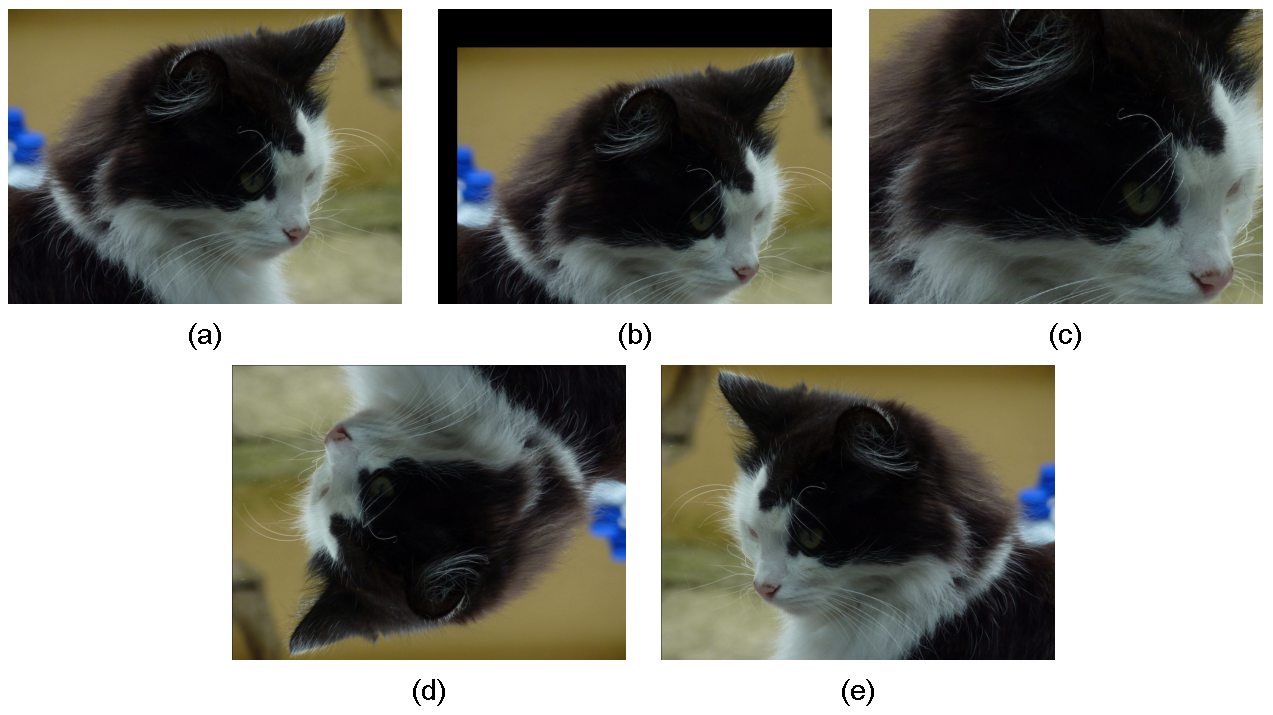
\includegraphics[width=0.5\textwidth]{imagens/PDI_Transformacoes_Geometricas.pdf}
\sourceAuthor
\label{fig:PDI_Transformacoes_Geometricas}
\end{figure}

\section{Segmentação de Regiões}
Conforme \cite{pedrini:2008} os métodos de segmentação de regiões detectam as regiões diretamente na imagem, ao invés de encontrar as bordas que delimitam as regiões. Os pontos apresentando propriedades similares são agrupados para formar uma região. Diversas propriedades podem ser usadas para caracterizar uma região, tal como intensidade de cinza, cor, informação semântica ou textura.

Os principais métodos de segmentação baseada em regiões podem ser classificados em crescimento de regiões, divisão de regiões, divisão e fusão de regiões e divisor de águas ou \textit{watersheds}.

\subsection{Crescimento de Regiões}

A segmentação baseada no crescimento de regiões se dá pela escolha de N pixels denominados sementes (ou \textit{seed}) onde, a partir deles, são crescidas as regiões anexando a cada ponto semente outros pixels que possuem propriedades similares. Os pixels semente podem ser escolhidos de forma aleatória, determinística ou empírica pelo usuário \cite{pedrini:2008}. O número de regiões segmentadas será sempre menor ou igual ao número de pontos sementes selecionados, mas nunca maior.

O predicado \(P\) a ser usado para agregar um pixel em uma das regiões verifica se a diferença absoluta entre os níveis de cinza desse pixel e o da semente é menor que um dado limitar \(T\), ou seja

\[P(R) = \left\{\begin{matrix}
\textup{VERDADEIRO}, & \textup{se }|f(x,y) - f(r,s)| \leq T\\ 
\textup{FALSO}, & \textup{caso contrário}
\end{matrix}\right.\]

em que \(f(r,s)\) representa o pixel semente e \(f(x,y)\) representa os pixels conectados ao pixel semente por vizinhança-8 \cite{pedrini:2008}. Qualquer pixel que satisfaça essa propriedade simultaneamente para ambas é (arbitrariamente) atribuído a região \(R_1\). 

\subsection{Divisão de Regiões}

Segundo \citet{pedrini:2008}, a segmentação baseada em divisão de regiões inicia-se com regiões formadas por pixels da imagem e, recursivamente, subdivide as regiões não-homogêneas em áreas menores. Em muitos casos, a imagem inteira pode ser considerada como uma região inicial. O processo de subdivisão termina quando todas as regiões satisfizerem o critério de similaridade.

Uma técnica comum de subdivisão da imagem em regiões homogêneas utiliza a representação quadtree, que é uma estrutura hierárquica baseada na decomposição recursiva e regular da imagem em quadrantes, de maneira que, para qualquer região \(R_i\), \(P(R_i) = \textup{VERDADEIRO}\). Ou seja, se \(P(R) = \textup{FALSO}\) então a imagem deve ser dividida em quadrantes. Se o predicado \(P\) for \(\textup{FALSO}\) para qualquer quadrante, o quadrante deve ser subdividido em subquadrantes e assim por diante \cite{pedrini:2008}.

\subsection{\textit{Watershed}}

Segundo \citet{pedrini:2008} o algoritmo de \textit{watershed} ou divisor de águas trata a imagem como se fosse uma superfície topográfica, onde as intensidades dos pixels correspondem a valores de altitude ou elevação. É efetuado então um processo chamado imersão onde os pontos de menor altitude (intensidade) passam a ser preenchidos de água, formando bacias. Quando duas bacias se encontram, uma linha de contenção é criada entre as bacias, definindo assim uma borda da imagem. O processo é executado até que toda a superfície tenha sido inundada.

\subsection{Afinamento de Bordas}

Conforme \citet{guilherme:2007} o processo de afinamento de bordas ou esqueletização consiste na remoção de pixels redundantes da imagem para a criação do seu esqueleto. O esqueleto de uma imagem é a representação básica das formas contidas na imagem, de forma que todos pixels são necessários. Os algoritmos de esqueletização sempre recebem como entrada uma imagem binarizada.

Uma das características mais importantes que define um bom algoritmo de esqueletização é a preservação das características das formas da imagem original. Estas características englobam posição, orientação, tamanho e conectividade \cite{guilherme:2007}.

\subsubsection{Stentiford}

O algoritmo de Stentiford foi proposto por \citet{stentiford:1983}, e adota uma abordagem baseada na utilização de máscaras para o afinamento de objetos. São utilizadas quatro máscaras que são aplicadas de forma sucessiva e ordenada \cite{guilherme:2007}. As máscaras são utilizadas para encontrar pixels na imagem que coincidam com um determinado padrão, sendo então marcados para remoção.

\begin{figure}[ht]
\centering
\caption{Máscaras utilizadas pelo algoritmo de Stentiford}
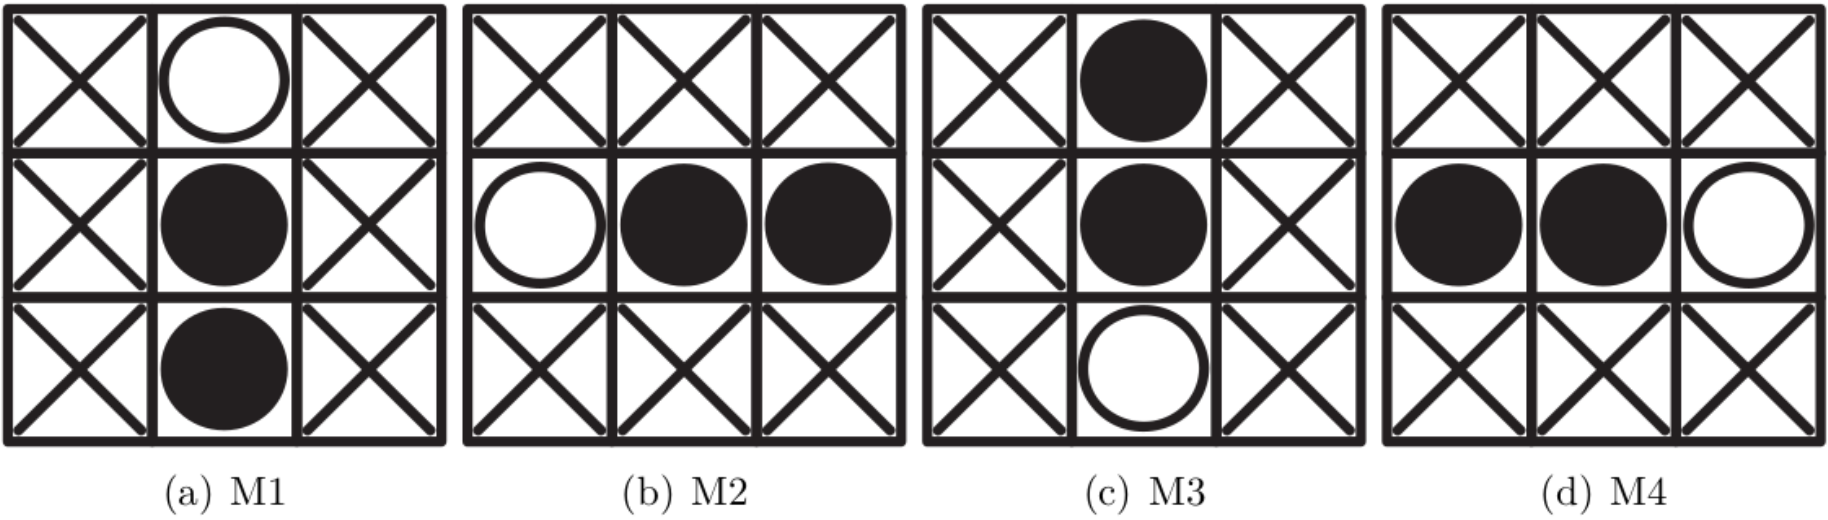
\includegraphics[width=0.8\textwidth]{imagens/PDI_Stentiford_1.PNG}
\source{\citet[pg.13]{guilherme:2007}}
\label{fig:PDI_Stentiford_1}
\end{figure}

Na Figura~\ref{fig:PDI_Stentiford_1} são demonstradas as máscaras utilizadas pelo algoritmo, onde os círculos brancos representam pixels de valor zero, os círculos pretos representam os pixels de valor 1 e os X representam os pixels com valores irrelevantes. Cada máscara percorre a imagem em uma determinada ordem: M1 da esquerda para a direita, de cima para baixo; M2 da esquerda para a direita, de baixo para cima; M3 da direita para a esquerda, de baixo para cima; e M4 da direita para a esquerda, de cima para baixo.

% TODO: Marta: E faz o que com isso???

\subsubsection{Zhang Suen}

O algoritmo de Zhang Suen \cite{zhang:1984} tem como base a comparação do pixel em processamento com seus 8 vizinhos. A exclusão de pixel por parte do algoritmo somente é realizada mediante a quatro regras. Estas regras têm como objetivo obter a exclusão segura dos pixels, garantindo, desta forma, que áreas interligadas não percam a conectividade e que a eliminação ocorrerá nas bordas do objeto \cite{guilherme:2007}.

\begin{figure}[ht]
\centering
\caption{Representa máscaras utilizadas pelo algoritmo de Zhang Suen}
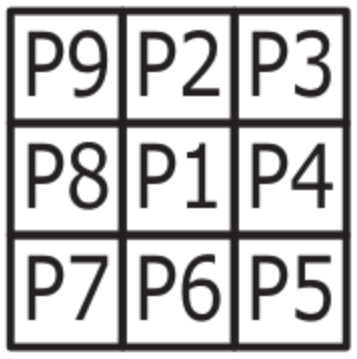
\includegraphics[width=0.3\textwidth]{imagens/PDI_Zhang_Suen_1.PNG}
\source{\citet[pg.15]{guilherme:2007}}
\label{fig:PDI_Zhang_Suen_1}
\end{figure}

O algoritmo é composto por duas iterações que fazem uso das quatro regras descritas na sequência. Na primeira iteração, para as regras C e D, serão utilizadas as máscaras descritas pela Figura~\ref{fig:PDI_Zhang_Suen_2} e Figura~\ref{fig:PDI_Zhang_Suen_3}, respectivamente, na segunda etapa, serão utilizadas as máscaras descritas pela Figura~\ref{fig:PDI_Zhang_Suen_4} e Figura~\ref{fig:PDI_Zhang_Suen_5}, respectivamente.

Segundo \citet{guilherme:2007}, para que um pixel seja marcado para exclusão ele deve:
\begin{itemize}
\item Possuir sua conectividade maior que 1;
\item O objeto deve ser composto de pelo menos dois e no máximo seis pixels pretos;
\item Ao menos um dos pixels da primeira máscara deve ser branco;
\item Ao menos um dos pixels da segunda máscara deve ser branco;
\end{itemize}

\begin{figure}[ht]
\centering
\caption{Pixels P2 ou P8 ou P4 devem ser um pixel branco}
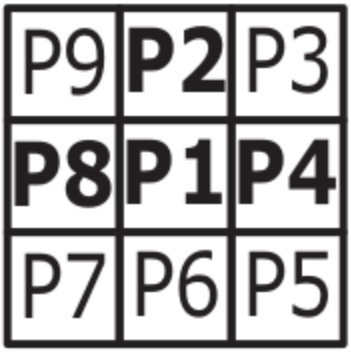
\includegraphics[width=0.3\textwidth]{imagens/PDI_Zhang_Suen_2.PNG}
\source{\citet[pg.16]{guilherme:2007}}
\label{fig:PDI_Zhang_Suen_2}
\end{figure}

\begin{figure}[ht]
\centering
\caption{Pixels P2 ou P8 ou P4 devem ser um pixel branco}
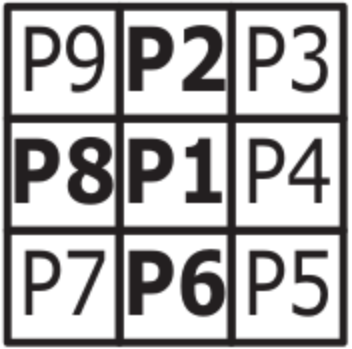
\includegraphics[width=0.3\textwidth]{imagens/PDI_Zhang_Suen_3.PNG}
\source{\citet[pg.16]{guilherme:2007}}
\label{fig:PDI_Zhang_Suen_3}
\end{figure}

\begin{figure}[ht]
\centering
\caption{Pixels P2 ou P4 ou P6 devem ser um pixel branco}
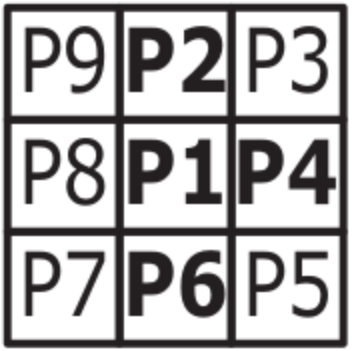
\includegraphics[width=0.3\textwidth]{imagens/PDI_Zhang_Suen_4.PNG}
\source{\citet[pg.16]{guilherme:2007}}
\label{fig:PDI_Zhang_Suen_4}
\end{figure}

\begin{figure}[ht]
\centering
\caption{Pixels P8 ou P6 ou P4 devem ser um pixel branco}
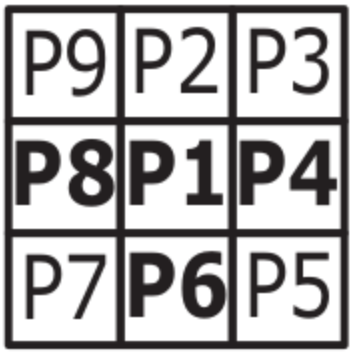
\includegraphics[width=0.3\textwidth]{imagens/PDI_Zhang_Suen_5.PNG}
\source{\citet[pg.17]{guilherme:2007}}
\label{fig:PDI_Zhang_Suen_5}
\end{figure}

\subsubsection{Holt}

O algoritmo de Holt \cite{holt:1987} utiliza uma vizinhança 3 x 3 para a análise dos pixels a serem removidos. O formato da matriz permite que seja feita uma análise do pixel central e seus vizinhos. Segundo \citet{guilherme:2007}, o algoritmo de Holt é composto por duas expressões lógicas, onde uma é aplicada na primeira iteração do algoritmo e a outra na segunda iteração.


Primeira iteração: 
\(v(C) \wedge (\sim edge(C) \vee (v(L) \wedge v(S) \wedge (v(N) \vee v(O))))\)

Segunda iteração:
\(v(C) \wedge (\sim edge(C) \vee (v(O) \wedge v(N) \wedge (v(S) \vee v(L))))\)

Para um ponto ser removido, o resultado das expressões lógicas devem ser verdadeiros. Nas expressões, os termos \(C\), \(O\), \(N\), \(S\) e \(L\) representam os vizinhos da imagem conforme definido na Figura~\ref{fig:PDI_Holt_1}. Já \(edge()\) e \(v()\) representam funções definidas por:
\begin{enumerate}
\item \(v()\): Retorna verdadeiro se o valor do ponto for o mesmo valor do objeto (valor preto) e falso se o valor do ponto for igual ao valor do plano de fundo (valor branco)
\item \(edge()\):Retorna verdadeiro se o valor processado estiver na borda do objeto e falso se não estiver
\begin{enumerate}[label*=\roman*.]
    \item Um pixel está na borda quando sua conectividade é igual a 1 e quando possuir de 2 a 6 vizinhos conectados
  \end{enumerate}
\end{enumerate}

\begin{figure}[ht]
\centering
\caption{Janela utilizada para a análise dos pixels vizinhos no algoritmo de Holt}
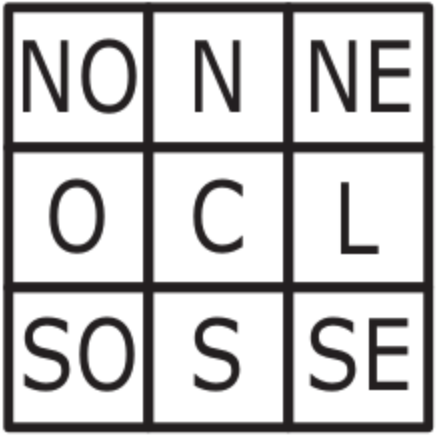
\includegraphics[width=0.3\textwidth]{imagens/PDI_Holt_1.PNG}
\source{\citet[pg.21]{guilherme:2007}}
\label{fig:PDI_Holt_1}
\end{figure}

\section{Considerações}

Este capítulo apresentou o tema de processamento digital de imagens. Foram apresentados os conceitos de imagem digital e as etapas de análise, como pré-processamento e segmentação. Além disso, foram apresentadas diversas técnicas de pré-processamento e segmentação, como \textit{thresholding}, detecção de bordas e morfologia matemática.

No próximo capítulo serão apresentadas trabalhos que tentaram unir o uso de algoritmos genéticos com PDI para realizar a segmentação de imagens digitais. Nos trabalhos indicados, o GA foi utilizado apenas para parametrizar as técnicas de PDI para alcançar o objetico especificado.

% ------------------------------------------------------------------------------------------------------------------------
\chapter{Trabalhos Correlatos}
% ------------------------------------------------------------------------------------------------------------------------

Neste capítulo serão apresentados trabalhos relacionados a área de pesquisa deste projeto.


\section{O Uso do Algoritmo Genético em Segmentação de Imagens Digitais}

A tese desenvolvida por \citet{matias:2007} aplica algoritmos genéticos com diferentes funções de avaliação para evoluir a parametrização de três métodos de segmentação de imagens digitais, comparando seu resultado. Os algoritmos de segmentação analisados são \textit{quadtrees}, limiarização e crescimento de regiões.

Todos os métodos visam minimizar uma função objetivo (entropia, segmentação excedente, entre outras) ou maximizar tal função (pixels corretamente agrupados). Para avaliação dos resultados, foram geradas várias imagens que utilizam o GA no algoritmo de segmentação e outras imagens geradas com o mesmo algoritmo, mas sem utilizar o GA. 

O método mais simples trabalhado por \citet{matias:2007} é a segmentação utilizando o limiar (\textit{threshold}). O objetivo dos AGs, neste tipo de algoritmo, é gerar de forma automática uma imagem segmentada por atribuição de um \textit{threshold}. A função de avaliação utilizada para este algoritmo foi a entropia.
% TODO: explicar o que ser entropia

Para a segmentação baseada em limiar a representação cromossômica foi utilizado um cromossomo de 8 genes binários, representando o valor do \textit{threshold} entre 0 e 255. 

Uma imagem utilizada para testes foi uma foto de 256x256 pixels denominada Lena. Para treinamento do GA foi utilizada uma população de 25 indivíduos, com uma probabilidade de mutação de 0.05 e uma probabilidade de \textit{crossover} de 0.6. O número máximo de gerações delimitado para o GA foi de 1000 gerações. A segmentação com a melhor função objetivo obtida por este método está exemplificada na Figura~\ref{fig:TrCo_Matias_Limiar_1}.

\begin{figure}[ht]
\centering
\caption{Resultado de limiarização na imagem Lena}
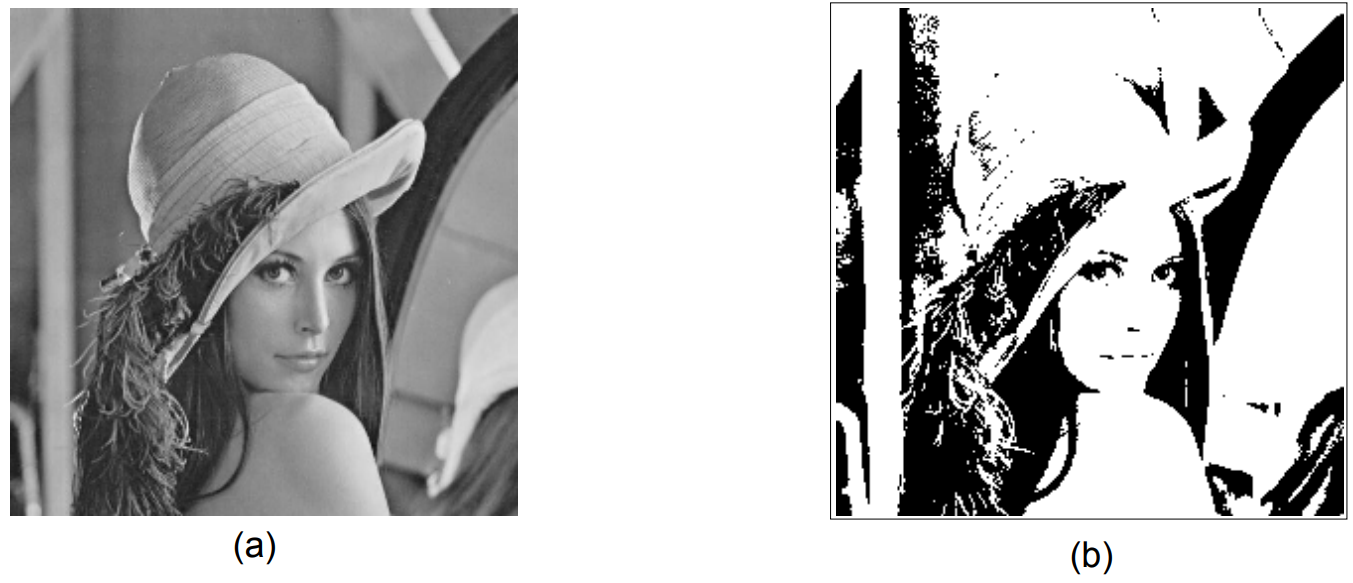
\includegraphics[width=0.7\textwidth]{imagens/TrCo_Matias_Limiar_1.PNG}
\source{\citet[Ppg.71]{matias:2007}}
\label{fig:TrCo_Matias_Limiar_1}
\end{figure}

Também foram realizados os mesmos testes utilizando uma foto de satélite do Rio Solimões em época de seca em alguns de seus afluentes. Utilizando os mesmos parâmetros do GA descritos anteriormente, a segmentação com melhor avaliação está demonstrada na Figura~\ref{fig:TrCo_Matias_Limiar_2}, onde também é demonstrado o uso do limiar ótimo descrito \cite{gonzalez:2012} (c).

\begin{figure}[ht]
\centering
\caption{Resultado de limiarização na imagem Rio Solimões}
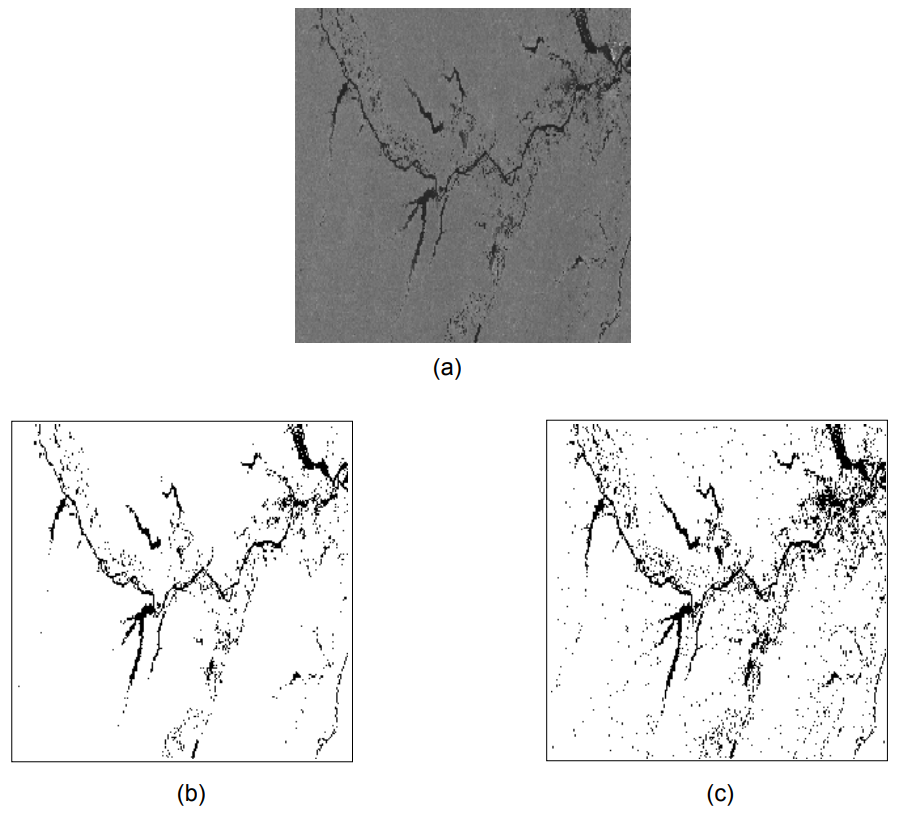
\includegraphics[width=0.7\textwidth]{imagens/TrCo_Matias_Limiar_2.PNG}
\source{\citet[pg.72]{matias:2007}}
\label{fig:TrCo_Matias_Limiar_2}
\end{figure}

Outro método implementado pela teste foi o método de segmentação por quadrantes, ou \textit{quadtree}. Neste método, o algoritmo genético foi utilizado para geração dos valores de entropia de cada nível da \textit{quatree}. Em uma imagem de resolução \(N\)x\(N\) pixels, o número de níveis representados por cada cromossomo é \(Lv=\log 2 N\). Cada valor do nível \(Lv_n\) representado no cromossomo indica o limiar de entropia daquele quadrante para que o mesmo seja subdividido novamente. O exemplo do cromossomo pode ser visto na Figura~\ref{fig:TrCo_Matias_Cromossomo_1}.

\begin{figure}[ht]
\centering
\caption{Cromossomo binário onde L corresponde a cada nível da quadtree}
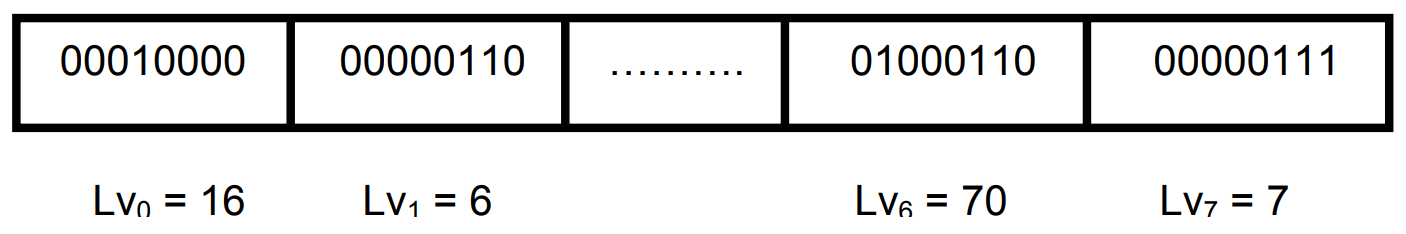
\includegraphics[width=0.8\textwidth]{imagens/TrCo_Matias_Cromossomo_1.PNG}
\source{\citet[pg.54]{matias:2007}}
\label{fig:TrCo_Matias_Cromossomo_1}
\end{figure}

Para validação da técnica de segmentação por \textit{quadtrees} foi utilizada a foto de satélite do Rio Solimões. A resolução da imagem é 256x256, o que gera uma Quadtree de 8 níveis. Para esta imagem foi executado o GA com uma população inicial aleatória de 300 indivíduos. A probabilidade de mutação utilizada foi de 0,1 e a probabilidade de \textit{crossover} foi de 0,6. A GA foi executada por um total de 9 gerações. O resultado da segmentação pode ser visto na Figura~\ref{fig:TrCo_Matias_Quadtree_1}. É possível identificar que a segmentação utilizando \textit{quadtrees} (c) e GAs foi mais eficiente que o método usual (b), gerando maiores áreas homogêneas, o que pode ser útil para compressão de imagens.

\begin{figure}[ht]
\centering
\caption{Comparação da segmentação via \textit{quadtree}}
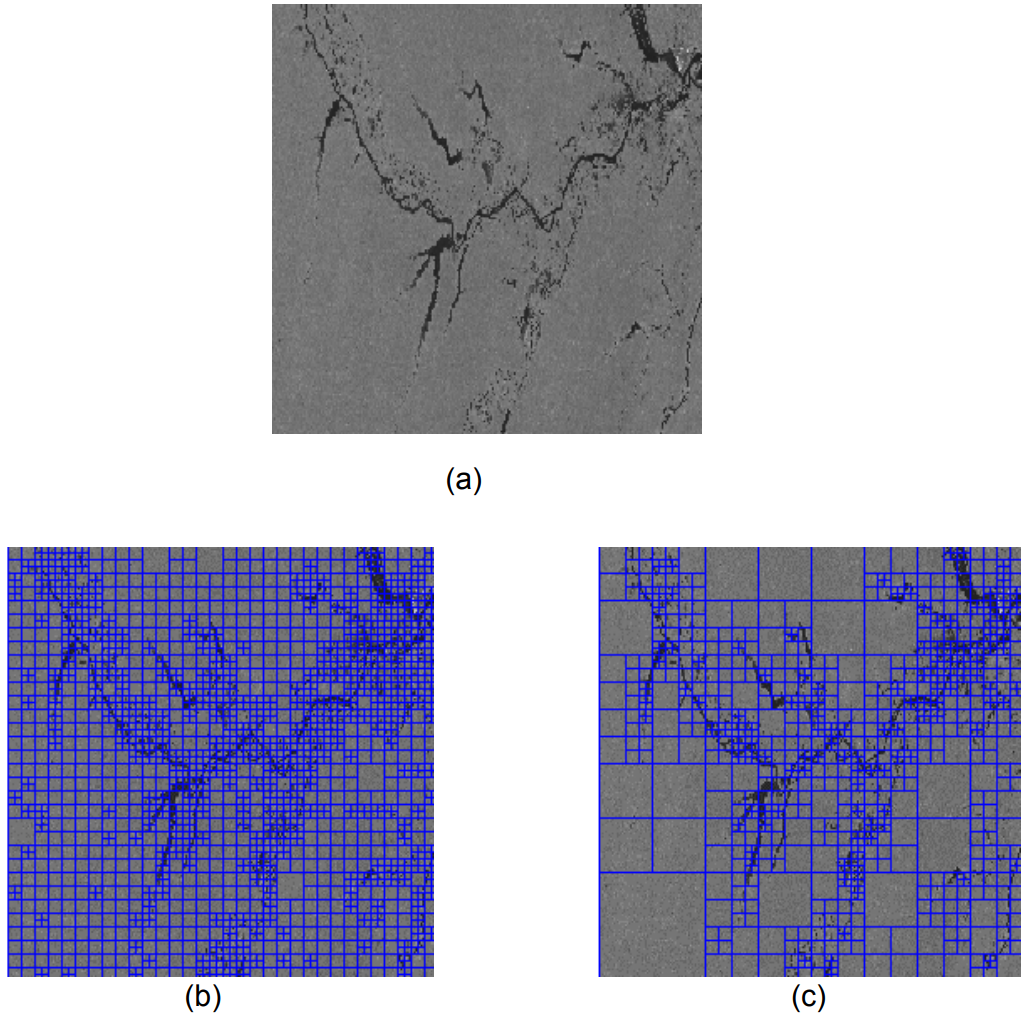
\includegraphics[width=0.6\textwidth]{imagens/TrCo_Matias_Quadtree_1.PNG}
\source{\citet[pg.68]{matias:2007}}
\label{fig:TrCo_Matias_Quadtree_1}
\end{figure}

Outro método de segmentação de imagens testado por \citet{matias:2007} foi o método de crescimento de regiões proposto por \citet{bins:1996}, um método que é direcionado a imagens de sensoriamento remoto. Este algoritmo utiliza dois parâmetros de entrada: o limiar de similaridade, utilizado para agrupar os pixels que estejam dentro deste valor, e a área máxima das regiões, para evitar problemas de \textit{under-segmentation}.

% TODO: Que métricas são essas?

A representação cromossômica deste método são os dois parâmetros de entrada concatenados em uma \textit{string} de \(K\) bits, onde \(K = \log_2 T + A\), sendo \(T\) o número máximo de tons de cinza da imagem e \(A\) um número suficiente de bits para armazenar a área máxima, neste caso \(A = 16\). Para validação do método, ao invés da entropia da imagem, foram utilizadas três métricas de avaliação de algoritmos de segmentação: CG, US e OS.

Para validação do processo de segmentação, foi utilizada uma foto de satélite de uma mancha de petróleo no mar, de resolução 256x256. Para a simulação do GA foi utilizada uma população de tamanho de 25 indivíduos aleatórios. A probabilidade de mutação utillizada foi de 0.05 e a probabilidade de \textit{crossover} foi de 0,6. O número máximo de gerações do GA foi de 1000. Ao final do processamento, foi obtida a saída representada na Figura~\ref{fig:TrCo_Matias_Crescimento_1}. Os valores do método de avaliação para a imagem segmentada sem GA (b) e com GA (c) pode ser visto na Tabela~\ref{tab:TrCo_Matias_1}.

\begin{figure}[ht]
\centering
\caption{Comparação da segmentação via crescimento de regiões}
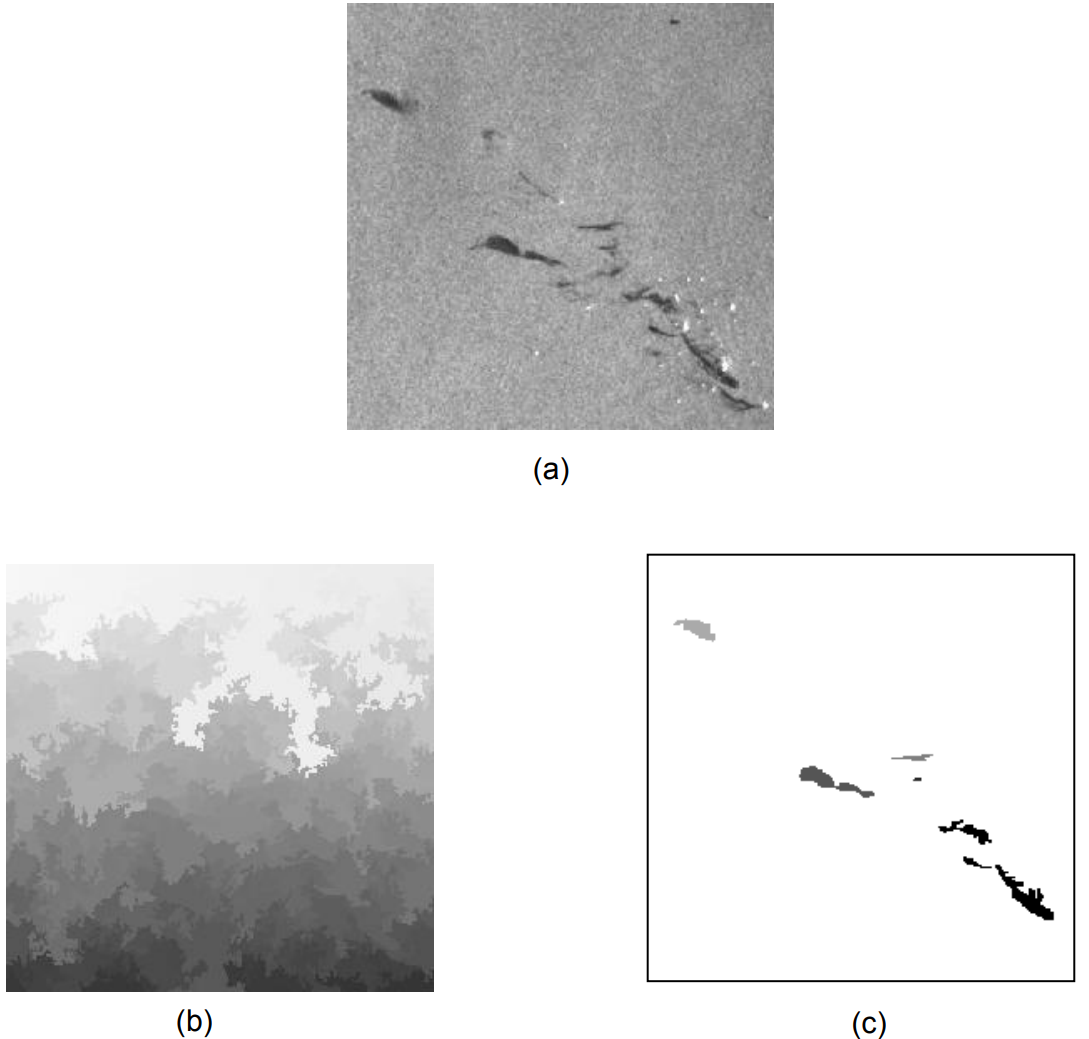
\includegraphics[width=0.6\textwidth]{imagens/TrCo_Matias_Crescimento_1.PNG}
\source{\citet[pg.68]{matias:2007}}
\label{fig:TrCo_Matias_Crescimento_1}
\end{figure}

\begin{table}
\centering
\caption{Resultados da segmentação}
\label{tab:TrCo_Matias_1}
\begin{tabular}{llll}
\hline
\multicolumn{1}{c}{\textit{\textbf{Caso}}} & \multicolumn{1}{c}{\textit{\textbf{CG}}} & \multicolumn{1}{c}{\textit{\textbf{US}}} & \multicolumn{1}{c}{\textit{\textbf{OS}}} \\ \hline
Sem GA                                     & 10,17\%                                  & 18,33\%                                  & 82,21\%                                  \\
Com GA                                     & 90,44\%                                  & 3,74\%                                   & 4,71\%                                   \\ \hline
\end{tabular}
\end{table}

Dessa maneira, \citet{matias:2007} verificou que o uso do GA com uma função objetivo adequada pode trabalhar muito bem em conjunto com algoritmos de segmentação, na busca de bons parâmetros de entrada iniciais. Isso foi comprovado nos três algoritmos testados: limiarização, \textit{quadtrees} e crescimento de regiões.

\section{A multilevel automatic thresholding method based on a genetic algorithm for a fast image segmentation}

Neste trabalho, \citet{hammouche:2008} propõem uma técnica de \textit{thresholding} multinível para a segmentação de imagens beasdo no uso de algoritmos genéticos para determinar os limiares apropriados. Segundo os autores, o uso de GAs tem várias vantagens sobre métodos de otimização tradicionais, particularmente a capacidade de encontrar a solução ótima global, prevenindo que o algoritmo fique preso em soluções localmente ótimas. Ademais, algoritmos genéticos podem ter uma grande redução no tempo de processamento com implementações paralelas. A técnica de \textit{thresholding} genética proposta é baseada em um GA padrão. Ele permite a determinação do número de limiares assim como o valor de cada um. 

Antes de realizar a busca dos limiares utilizando o GA, o tamanho do histograma da imagem é reduzido de forma a acelerar a convergência do GA. A redução do histograma é feita utilizando a técnica de \textit{wavelet transform} \cite{kim:2003}. O histograma é reduzido para dois sinais. O primeiro é o sinal de tendência, ou sinal de aproximação, enquando o segundo é o sinal de detalhe.

No GA proposto, o cromossomo é codificado como uma String binária \(A\) com o mesmo comprimento do histograma reduzido \(L^r\), se forma que \(A = a_0, a_1, ... a_{L^r-1}\), onde o gene \(a_i\) possui o valor 0 ou 1, representando se o índice é um pico ou um vale no histograma, respectivamente. A posição \(i\) onde \(a_i = 0\) indica o valor onde existirá um \textit{threshold}. Dessa forma, o número de \textit{bits} 0 no cromossomo indica o número de limiares.

Para permitir a solução ótima do número de \textit{thresholds} e seus valores, a função objetiva é calculada usando a função de custo ACT proposta por \citet{yen:1995}. Esta função avalia a entropia de cada classe criada, levando em consideração o número de limiares utilizados. Com este método, é garantida a segmentação boa da imagem utilizando um número tão pequeno quanto possível de limiares.

A população do algoritmo genético é inicializada com uma população gerada aleatóriamente de individuos. Para a avaliação do GA, o indivíduo com a melhor função objetivo em cada geração é copiada para uma posição isolada da população de forma a armazenar a melhor solução atual. Então, antes de começar a próxima geração, a melhor solução pode melhorar a sua avaliação realizando diversas pequenas modificações em seus genes. Esta simples técnica pode economizar diversas várias gerações de aprimoramento e não afeta o comportamento geral do GA.

A população corrente evolui para a próxima geração utilizando as três técnicas padrões de GAs: seleção, \textit{crossover} e mutação. Para a seleção, é utilizada a técnica da roleta viciada. Para o \textit{crossover}, é utilizado o método de ponto único. Também é utilizada a mutação tradicional. Após o \textit{crossover} e mutação, o novo gene pode conter uma sequência de vários \textit{bits} 0 seguidos, o que não é desejável. Para evitar essa sitação, é realizado um ajuste no cromossomo de forma que apenas o primeiro zero sucessivo é mantido, trocando os subsequentes pelo valor 1.

Para a validação dos resultados, foram utilizadas algumas imagens comumente utilizadas para validação de técnicas de processamento de imagens: \textit{Lena}, \textit{Blood}, \textit{Peppers}, \textit{House}, \textit{Airplane}, \textit{Lac}, \textit{Boats} e \textit{Bridge}. Na Figura X estão demonstradas as figuras utilizadas tal como o resultado da segmentação das imagens. Os resultados obtidos provam a robustez do método proposto, no aspecto de acurácia na segmentação. Uma comparação dos resultados da imagem Lena podem ser vistos na Tabela~\ref{tab:TrCo_Bammouche_Resultados}.

\begin{table}[]
\centering
\caption{Comparação do métoodo proposto com outros métodos semelhantes}
\label{tab:TrCo_Bammouche_Resultados}
\begin{tabular}{llllll}
\hline
\textit{\textbf{\small{Método}}} & \textit{\textbf{\small{Classes}}} & \textit{\textbf{\small{Valores limiares}}} & \textit{\textbf{\small{FA}}} & \textit{\textbf{\small{Uniformidade}}} & \textit{\textbf{\small{Tempo (ms)}}} \\ \hline
ES-Otsu                  & 5                                   & 47-84-119-164                          & 10,80                           & 0,97877                        & 601.766                             \\
ES-Kapur                 & 4                                   & 60-109-160                             & 11,00                           & 0,97159                        & 50.281                              \\
GA-Otsu                  & 5                                   & 46-80-113-162                          & 10,82                           & 0,97805                        & 578                                 \\
GA-Kapur                 & 4                                   & 59-107-159                             & 10,97                           & 0,97177                        & 1.118                               \\
Iterative-Otsu           & 5                                   & 47-83-118-163                          & 10,80                           & 0,97874                        & 360                                 \\
Iterative-Kapur          & 4                                   & 60-108-159                             & 10,99                           & 0,97160                        & 1516                                \\
Método proposto          & 5                                   & 46-83-119-164                          & 10,80                           & 0,97875                        & 32                                  \\ \hline
\end{tabular}
\end{table}

% ------------------------------------------------------------------------------------------------------------------------
\chapter{Proposta}
% ------------------------------------------------------------------------------------------------------------------------

Neste trabalho é proposto um sistema de aprendizado de máquina utilizando algoritmos genéticos com técnicas de processamento digital de imagens para segmentação de imagens, focando na segmentação de fotos de rostos. De forma semelhante aos trabalhos apresentados como correlatos, os GAs serão utilizados para evoluir os parâmetros das técnicas de processamento de imagem. No entanto, o principal objetivo deste trabalho é conseguir que o GA selecione também quais técnicas de PDI e em qual sequência os mesmos serão executados para obter o melhor resultado do processo de segmentação.

Este trabalho se baseia no \textit{software} VISNode \cite{visnode:2018}, uma ferramenta para execução de técnicas de PDI em formato de grafo. Ele possui dezenas de algoritmos de PDI implementados que serão utilizados neste trabalho. Cada nodo possui entradas e saídas, sendo que estas podem ser conectadas entre si, garantindo uma maior flexibilidade no sequenciamento e execução dos algoritmos. Um exemplodo de um projeto do VISNode com 7 nodos (processos) de PDI pode ser visto na Figura~\ref{fig:PRO_Visnode}.

\begin{figure}[ht]
\centering
\caption{Demonstração de um processo feito no VISNode}
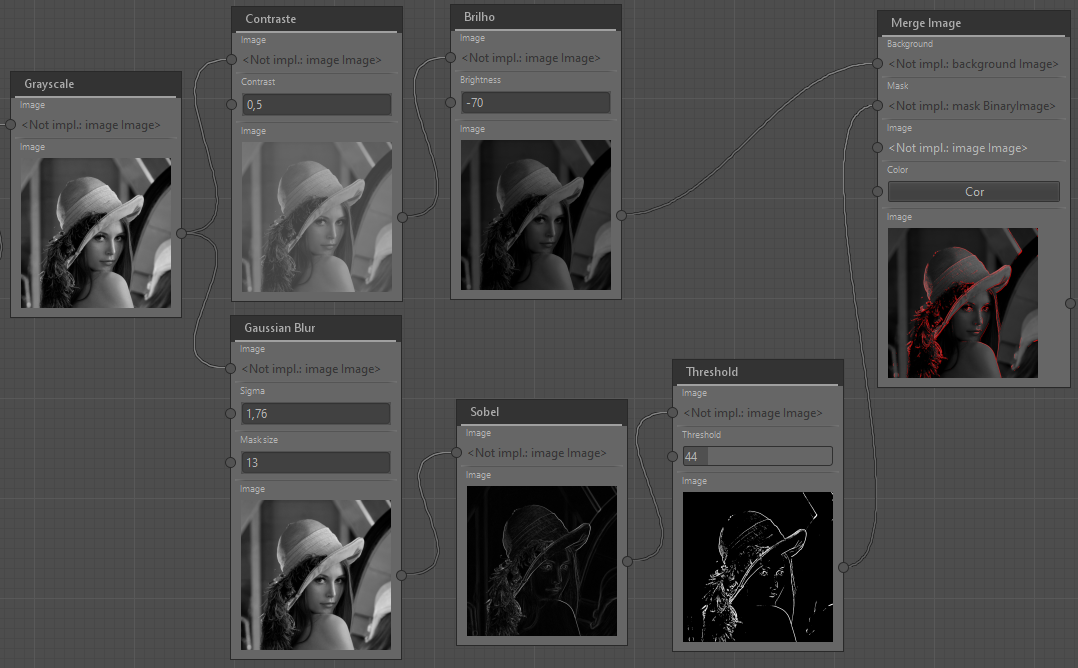
\includegraphics[width=0.8\textwidth]{imagens/PRO_Visnode.PNG}
\sourceAuthor
\label{fig:PRO_Visnode}
\end{figure}

% TODO: Figura
No GA proposto, cada indivíduo representará um grafo de processos de PDI, permitindo a parametrização estática (valor fixo para o parâmetro) ou dinâmica (vindo de outro nodo do grafo) de cada algoritmo. Como exemplo de possíveis indivíduos do GA, podemos citar:
\begin{itemize}
    \item execução da detecção de bordas de Sobel, seguida de uma limiarização e a execução do algoritmo de \textit{Snakes} para preenchimento das regiões;
    \item obtém a média dos tons de cinza da imagem e utiliza isso como limiar para o processo de \textit{thresholding};
    \item a imagem ainda colorida está sendo dividida em três imagens tons de cinza baseadas nos seus canais RGB, é efetuado um limiar fixo em cada uma delas, para então se unir os conjuntos gerados
\end{itemize}

Para avaliação dos indivíduos do GA e validação do trabalho, está sendo utilizada a base de rostos segmentados FASSEG \cite{fasseg:2018}. Esta base possui 70 fotos de rostos normalizados (com posição e iluminação semelhantes) e as imagens já segmentadas delineando o rosto, olhos, cabelo, boca e nariz em cores diferentes. Exemplos de imagens de entrada e segmentadas podem ser vistos na Figura ~\ref{fig:FASSEG}. Neste trabalho o objetivo principal é que seja possível segmentar de forma satisfatória o contorno do rosto, ou seja, sem o fundo e sem os cabelos, mas contendo olhos e boca.

\begin{figure}[ht]
\centering
\caption{Exemplo de imagens do FASSEG}
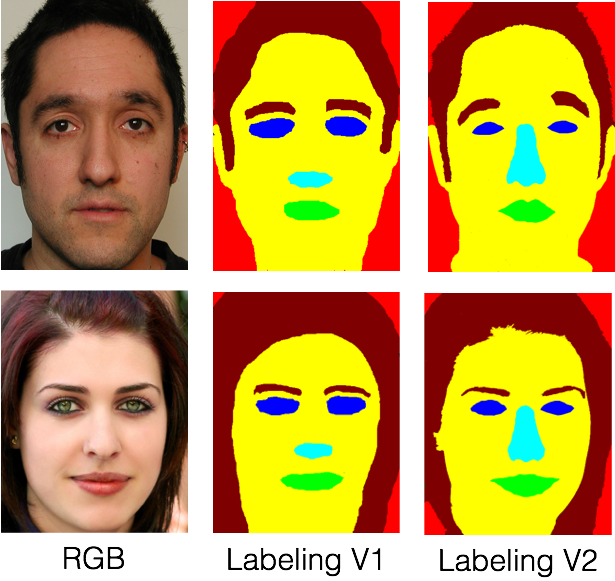
\includegraphics[width=0.6\textwidth]{imagens/FASSEG.png}
\source{\citet{fasseg:2018}}
\label{fig:FASSEG}
\end{figure}

O método para validação das imagens é uma simples comparação pixel a pixel da imagem gerada pelo GA com a imagem pré-segmentada do FASSEG. Com uma imagem de entrada da base selecionada, o método gerado pelo GA é executado, gerando sempre uma imagem binária. Esta imagem é então comparada com a imagem pré-segmentada da base, contando o número de pixels corretos \(c\). Este número é então dividido pelo número total de pixels de imagem \(t\), dando a função objetivo \(F\), que representa o percentual de asserção deste indivíduo. Dessa forma, \(F\) pode ser definido como \(F = \frac{c}{t}\).

\section{Representação cromossomial}

Uma das partes mais importantes do trabalho é a definição da representação cromossomial dos grafos. Em um único cromossomo deve ser possível codificar um conjunto de nodos, cada nodo possuindo um processo a ser executado (categórico), e 0-N parâmetros numéricos. Além disso, deve ser possível codificar no cromossomo as conexões entre os nodos do grafo.

\section{Processos de PDI}

Cada nodo do grafo representado por cada indivíduo possui um processo vinculado a si. Esse processo pode ser um de diversos algoritmos de PDI disponibilizados pelo \textit{framework} do VISNode, ou ainda alguns outros operadores auxiliares (também disponíveis no \textit{framework}), como operadores matemáticos (soma, subtração, multiplicação, etc) e operadores de filtragem (maior objeto, menor objeto, etc).

\section{Definição do GA}

Para construção do algoritmo genético serão usados os indicados pela literatura, sendo eles mutação, \textit{crossover} e seleção por roleta viciada. Serão testadas algumas variações destes métodos, como \textit{crossover} de um ponto, dois pontos ou uniforme e roleta viciada normalizada, selecionando aqueles que trouxerem o melhor resultado. Também serão testadas variações dos parâmetros do GA, como taxa de mutação e taxa de \textit{crossover}, a fim de otimizar os resultados encontrados.

% ------------------------------------------------------------------------------------------------------------------------
\chapter{Desenvolvimento}
% ------------------------------------------------------------------------------------------------------------------------

\section{Teste 1}

No início do desenvolvimento deste trabalho, foi construído um protótipo para avaliar a viabilidade da proposta. O intuito deste teste era implementar um GA para evolução de técnicas de PDI e seus parâmetros para realizar a segmentação de uma única imagem (\textit{overfitting}).

Para o teste, foi selecionada uma imagem de um rosto da base de imagens FASSEG \cite{fasseg:2018}. Para avaliação da imagem, foi realizada a comparação pixel a pixel da imagem de saída do GA com o gabarito disponível na base.

Nesta fase, o cromossomo era composto de 21 genes, divididos em 7 grupos de 3 genes. O primeiro gene de cada grupo indicava qual técnica de PDI deveria ser utilizada, e os outros 2 genes possuem parâmetros para a execução do algoritmo. O GA poderia escolher entre sete algoritmos de PDI diferentes, demonstrados na Tabela~\ref{tab:AlgoritmosTeste1}.

\begin{table}
\centering
\caption{Algoritmos utilizados}
\label{tab:AlgoritmosTeste1}
\begin{tabular}{ll}
\hline
\textit{\textbf{Algoritmo}}  & \textit{\textbf{Parâmetros}}                                                           \\ \hline
Conversão para tons de cinza & -                                                                                      \\ 
Limiarização                 & {[}1{]} Limiar, 0-255                                                                  \\ 
Inversão de cores            & -                                                                                      \\ 
Ajuste de brilho             & {[}1{]} Brilho, -255 -255                                                              \\ 
Ajuste de contraste          & {[}1{]} Contraste, 0 - 3                                                               \\ 
Filtor de mediana            & -                                                                                      \\ 
Filtro gaussiano             & \begin{tabular}[c]{@{}l@{}}{[}1{]} Sigma, 0 - 3;\\ {[}2{]} Máscara, 3 - 11\end{tabular} \\ \hline
\end{tabular}
\end{table}

Para a execução do GA, foi utilizada uma população de tamanho 150, e o mesmo foi executado por 100 gerações. Ao final da execução, a melhor solução encontrada possui uma avaliação de 0,9692, ou seja, 96,92\% de assertividade com o gabarito. O resultado final do algoritmo pode ser visto na Figura~\ref{fig:DES_Primeiro_Teste}.

\begin{figure}[ht]
\centering
\caption{Resultado do primeiro teste}
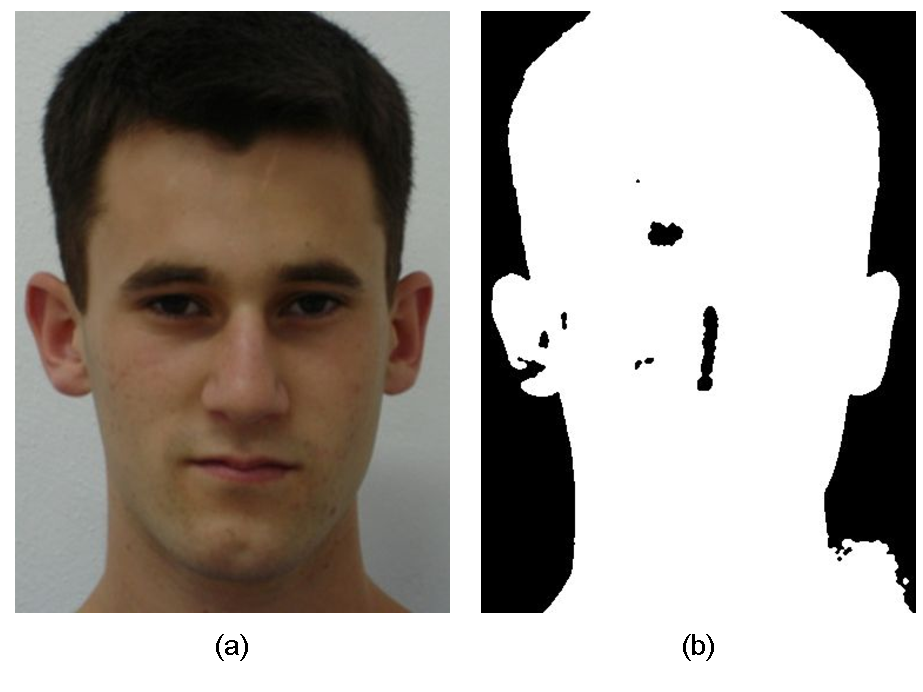
\includegraphics[width=0.6\textwidth]{imagens/DES_Primeiro_Teste.pdf}
\sourceAuthor
\label{fig:DES_Primeiro_Teste}
\end{figure}

Foi identificada uma rápida convergência para o resultado final, devido a simplicidade do problema e ao pequeno espaço de possíveis soluções. Na primeira geração, completamente aleatória, já estava presente o cromossomo com 96,92\% de assertividade, que foi o sobrevivente até o final da 100ª geração. Ao decorrer do processo, os seus genes foram se espalhando pela população, e não houve melhoria devida a mutação.

\section{Teste 2}

O segundo teste foi focado em adicionar mais processos para tentar melhorar o percentual de assertividade do GA. Foram adicionados 15 algoritmos aos 7 já adicionados no primeiro teste. Além disso, existe a possibilidade do processo ser um processo de terminação, o que possibilita um número variável de processos em cada gene. Os novos 16 processos adicionados estão na Tabela~\ref{tab:AlgoritmosTeste2}.

%TODO: Preencher
\begin{table}
\centering
\caption{Algoritmos utilizados}
\label{tab:AlgoritmosTeste2}
\begin{tabular}{ll}
\hline
\textit{\textbf{Algoritmo}}  & \textit{\textbf{Parâmetros}}                                                           \\ \hline
Tons de cinza ponderados     & \begin{tabular}[c]{@{}l@{}}{[}1{]} Peso R, 0 - 1;\\ {[}2{]} Peso G, 0 - 1\\ {[}2{]} Peso B, 0 - 1\end{tabular} \\ 
Erosão                       & -                                                                                      \\ 
Dilatação                    & -                                                                                      \\ 
Abertura                     & -                                                                                      \\ 
Fechamento                   & -                                                                                      \\ 
Sobel                        & -                                                                                      \\ 
Roberts                      & -                                                                                      \\ 
Robinson                     & -                                                                                      \\ 
Prewitt                      & -                                                                                      \\ 
Canny                        & -                                                                                      \\ 
Snake                        & -                                                                                      \\ 
Stentiford                   & -                                                                                      \\ 
Zhang Suen                   & -                                                                                      \\ 
Holt                         & -                                                                                      \\ 
Desfoque com média           & -                                                                                      \\  \hline
\end{tabular}
\end{table}

Cada cromossomo foi incrementado para um tamanho de 36 genes, (9 grupos de 4), permitindo a execução de até 9 processos em sequência. Também foi alterado o processo de seleção com relação ao primeiro teste, realizando a técnica da roleta viciada inversa para que os melhores indivíduos de cada geração tenham uma chance de sobreviver até a próxima geração. O tamanho da população foi incrementado para 300, devido ao aumento do espaço de soluções possíveis.

O teste agora foi executado em três imagens da base FASSEG ao invés de apenas uma, com o objetivo de tentar encontrar uma solução mais genérica para o problema da segmentação. Após a execução do algoritmo por 100 gerações, o melhor resultado da segmentação foi de 65,23\% (Média de assertividade entre as três imagens). O exemplo da saída do algoritmo esta na Figura~\ref{fig:DES_Segundo_Teste}.

\begin{figure}[ht]
\centering
\caption{Resultado do segundo teste}
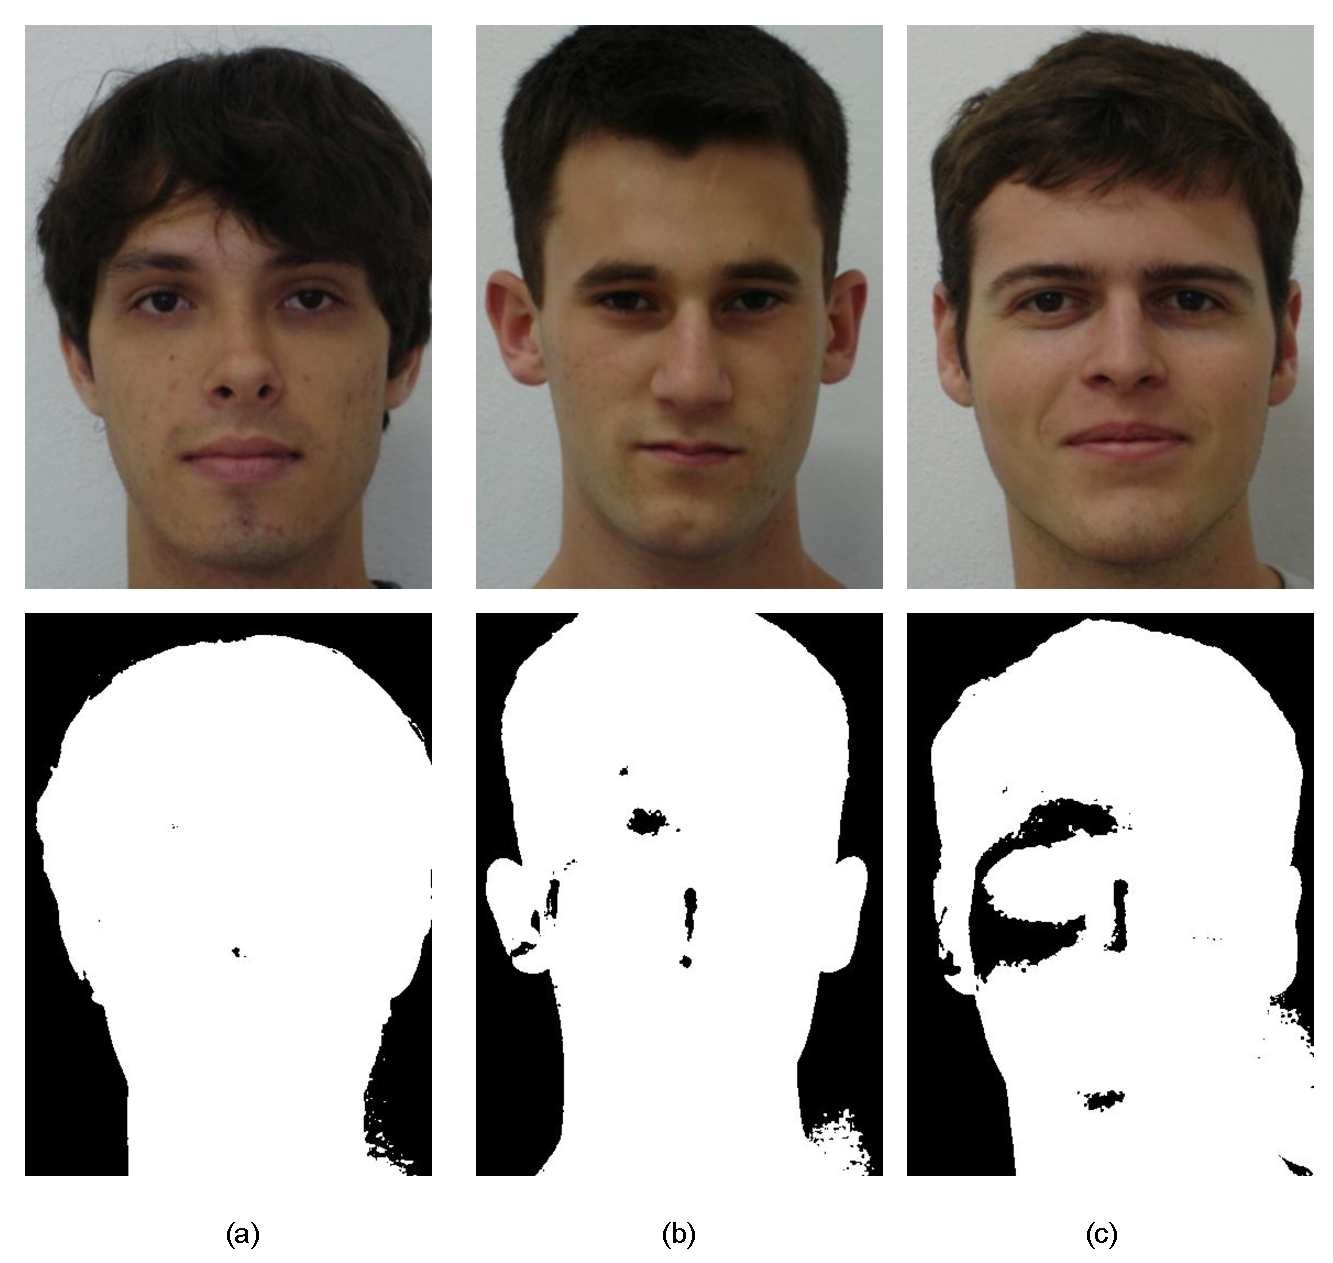
\includegraphics[width=0.6\textwidth]{imagens/DES_Segundo_Teste.pdf}
\sourceAuthor
\label{fig:DES_Segundo_Teste}
\end{figure}

Com esse teste foi possível verificar alguns problemas com a abordagem atual:
\begin{itemize}
    \item Todos os indivíduos bem sucedidos usam o \textit{thresholding}, o que não é ideal;
    \item Está se perdendo muita diversidade genética sem obter melhorias nos melhores indivíduos;
    \item Alguns indivíduos tiveram um percentual extremamente baixo (0,4\%), o que, na verdade, significa que ele gerou algo semelhante ao negativo da melhor solução.
\end{itemize}

No primeiro problema, onde o único método bem sucedido é o \textit{thresholding}, foi identificado que soluções que utilizam métodos de detecção de bordas não tem um resultado bom pois não possuem um método para preenchimento da borda gerada. Para solucionar este problema, serão disponibilizados processos de preenchimento, como o \textit{Flood Fill}. Além disos, serão criados processos de segmentação baseados em regiões, aumentando o conjunto de soluções possíveis.

Para solucionar o segundo problema, serão realizados testes sem utilizar valores fixos para a taxa de \textit{crossover} e mutação, ajustando os mesmos conforme a execução do algoritmo.

O terceiro problema será resolvido considerando imagens que geraram o negativo do gabarito como soluções também muito boas. Isso será feito considerando que a função de avaliação \(a\) será \(a = 1 - a\) caso a mesma seja menor que 0,5.

% ---
% Finaliza a parte no bookmark do PDF, para que se inicie o bookmark na raiz
% ---
\bookmarksetup{startatroot}% 
% ---

% ---
% Conclusão
% ---
\chapter{Conclusão}
\addcontentsline{toc}{chapter}{Conclusão}

% ----------------------------------------------------------
% ELEMENTOS PÓS-TEXTUAIS
% ----------------------------------------------------------
\postextual


% ----------------------------------------------------------
% Referências bibliográficas
% ----------------------------------------------------------
\bibliography{abntex2-modelo-references}


%---------------------------------------------------------------------
% INDICE REMISSIVO
%---------------------------------------------------------------------

\printindex

\end{document}
d